\chapter{Diffusion and flexible Graph Networks}

%==============================================================================
%
%==============================================================================
\section{Diffusion Networks}

%------------------------------------------------------------------------------
%
%------------------------------------------------------------------------------
\subsection{Introduction}

Diffusion models represent a class of generative neural networks that have recently achieved remarkable success in areas such as image generation (e.g., DALL\textperiodcentered E 2, Stable Diffusion) and molecular design. Their core principle is inspired by physical diffusion processes: transforming data into noise and learning to reverse this process. In this way, diffusion models learn to generate new data samples from pure noise through a learned denoising process.

In the context of weather and climate, diffusion models offer a new paradigm for generative modeling, ensemble forecasting, and uncertainty quantification. Traditional numerical weather prediction (NWP) relies on the integration of physical models forward in time, often facing challenges in representing uncertainty and producing diverse ensemble members. Diffusion models can be used as a complementary or alternative strategy: they learn the statistical structure of weather or climate fields and generate samples that respect these statistics, conditioned on given observations or coarse-resolution forecasts.

This section introduces the core ideas and mathematical framework of diffusion models, with a focus on applications to geophysical data.

%------------------------------------------------------------------------------
%
%------------------------------------------------------------------------------
\subsection{Forward and Reverse Diffusion Processes}

%------------------------------------------------------------------------------
%
%------------------------------------------------------------------------------
\subsubsection{The Forward Process (Adding Noise)}

Let $\mathbf{x}_0 \in \mathbb{R}^d$ be a sample from the true data distribution (e.g., a temperature field, wind vector, or other atmospheric variable on a spatial grid). The forward diffusion process corrupts $\mathbf{x}_0$ over $T$ discrete time steps by gradually adding Gaussian noise, producing a sequence of increasingly noisy samples $\mathbf{x}_1, \dots, \mathbf{x}_T$.

\begin{figure}[htbp]
    \centering
    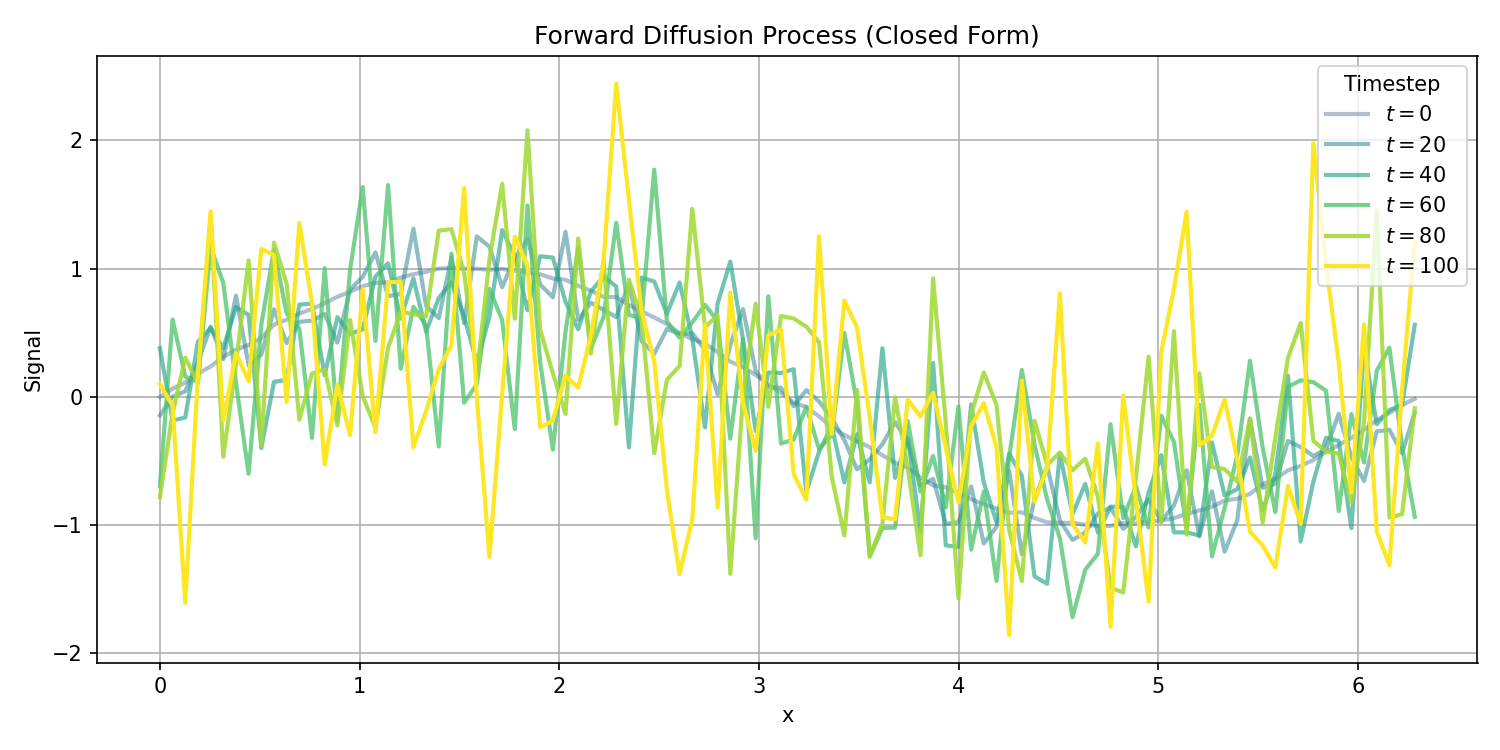
\includegraphics[width=0.9\textwidth]{images/diffusion1.png}
    \caption{
        Forward diffusion process applied to a sine function over 101 steps.
        Every 20th step is shown with increasing transparency and brightness.
        Initially, the signal is clean (\( t=0 \)), and as the diffusion progresses,
        Gaussian noise increasingly dominates the structure. The process is
        governed by a predefined noise schedule using a cumulative variance
        parameter \( \bar{\alpha}_t \), ensuring that \( \mathbf{x}_t \) converges
        toward a standard Gaussian distribution as \( t \rightarrow T \).
    }
    \label{fig:diffusion-forward}
\end{figure}


This process is modeled as a Markov chain:

$$
q(\mathbf{x}_1, \dots, \mathbf{x}_T | \mathbf{x}_0) = \prod_{t=1}^T q(\mathbf{x}_t | \mathbf{x}_{t-1}),
$$

where each transition adds noise as:

$$
q(\mathbf{x}_t | \mathbf{x}_{t-1}) = \mathcal{N}(\mathbf{x}_t; \sqrt{1 - \beta_t} \mathbf{x}_{t-1}, \beta_t \mathbf{I}).
$$
Here, each component in the Gaussian transition
\[
q(\mathbf{x}_t \mid \mathbf{x}_{t-1}) = \mathcal{N}\left(\mathbf{x}_t;\, \sqrt{1 - \beta_t} \, \mathbf{x}_{t-1},\, \beta_t \mathbf{I} \right)
\]
has the following role and dimensional interpretation:
\begin{itemize}
    \item \( \mathbf{x}_t \in \mathbb{R}^d \) is the noisy variable at step \( t \), drawn from the distribution.
    \item The mean of the Gaussian is \( \boldsymbol{\mu}_t = \sqrt{1 - \beta_t} \, \mathbf{x}_{t-1} \in \mathbb{R}^d \), which scales the previous state downward. This reduces the signal amplitude as noise is added, ensuring the data gradually diffuses toward a Gaussian distribution.
    \item The covariance is \( \boldsymbol{\Sigma}_t = \beta_t \mathbf{I} \in \mathbb{R}^{d \times d} \), where \( \mathbf{I} \) is the identity matrix. This defines isotropic Gaussian noise with variance \( \beta_t \) in each dimension.
    \item \( \beta_t \in (0, 1) \) is a predefined noise schedule that increases over time. Small values at early steps retain more structure; larger values at later steps ensure full noise.
\end{itemize}

As \( t \to T \), the distribution of \( \mathbf{x}_t \) converges to the standard normal distribution \( \mathcal{N}(0, \mathbf{I}) \), effectively transforming structured data into pure noise.


As $t \to T$, the sample $\mathbf{x}_T$ approaches pure Gaussian noise: $\mathcal{N}(0, \mathbf{I})$.
This process is fixed and does not involve learning. It provides synthetic training pairs $(\mathbf{x}_t, t, \mathbf{x}_0)$ to train the reverse model.

%------------------------------------------------------------------------------
%
%------------------------------------------------------------------------------
\subsubsection{The Reverse Process (Learning to Denoise)}

The generative aspect of diffusion models lies in the reverse process, which seeks to map noise back to data. This process is defined by:

$$
p_\theta(\mathbf{x}_{0:T}) = p(\mathbf{x}_T) \prod_{t=1}^T p_\theta(\mathbf{x}_{t-1} | \mathbf{x}_t),
$$

where:
\begin{itemize}
\item $p(\mathbf{x}_T) = \mathcal{N}(0, \mathbf{I})$ is the assumed prior distribution (pure noise),
\item $p_\theta(\mathbf{x}_{t-1} | \mathbf{x}_t)$ is the learned denoising distribution parameterized by a neural network.
\end{itemize}

The network predicts a mean $\mu_\theta(\mathbf{x}_t, t)$ and often assumes a fixed variance $\Sigma_t$, resulting in:

$$
p_\theta(\mathbf{x}_{t-1} | \mathbf{x}_t) = \mathcal{N}(\mathbf{x}_{t-1}; \mu_\theta(\mathbf{x}_t, t), \Sigma_t).
$$

The denoising network can be conditioned on additional inputs such as class labels, spatial information, or physical constraints, making it suitable for structured data like weather fields.

%------------------------------------------------------------------------------
%
%------------------------------------------------------------------------------
\subsection{Loss Function and Training}

In the denoising framework used here, the neural network is trained to predict a less noisy version of the input, i.e., an estimate of \( \mathbf{x}_{t-1} \) given the current noisy state \( \mathbf{x}_t \) and conditioning information (e.g., class or weather constraints).

At each training step, we use a sequence of noisy inputs generated from a known clean signal \( \mathbf{x}_0 \), perturbed by Gaussian noise through the forward process. The training loss at each denoising step is given by the mean squared error:

\[
\mathcal{L}_t(\theta) = \mathbb{E}_{\mathbf{x}_{t}, \mathbf{x}_{t-1}} \left[ \left\| \mathbf{x}_{t-1} - f_\theta(\mathbf{x}_t, t, \text{cond}) \right\|^2 \right],
\]

where:
\begin{itemize}
    \item \( \mathbf{x}_t \in \mathbb{R}^d \) is the noisy state at time \( t \),
    \item \( \mathbf{x}_{t-1} \in \mathbb{R}^d \) is the target (previous, less noisy) state,
    \item \( f_\theta(\cdot, t, \text{cond}) \) is the neural network that predicts the denoised state, possibly conditioned on class labels or physical context,
    \item The expectation is taken over randomly sampled timesteps and training examples.
\end{itemize}

The total loss is averaged over all reverse steps from \( t = T \) to \( 1 \). This approach turns denoising into a stepwise regression problem toward the clean signal trajectory, rather than estimating the noise directly as in DDPM.

%------------------------------------------------------------------------------
%
%------------------------------------------------------------------------------
\subsection{Relevance to Weather and Climate}

In weather and climate science, data is high-dimensional, often spatial-temporal, and exhibits strong structure (e.g., physical constraints, correlations, seasonal cycles). Diffusion models are particularly suited to such domains because they:

\begin{itemize}
\item Learn \textbf{nonlinear distributions} of full fields (e.g., 2m temperature, geopotential height),
\item Allow \textbf{conditional generation}, e.g., generating high-resolution forecasts conditioned on coarse-resolution inputs,
\item Support \textbf{stochastic generation}, producing diverse ensemble members,
\item Can be guided or constrained by physical priors or observations.
\end{itemize}

Recent applications include:
\begin{itemize}
\item Generating ensemble weather forecast members,
\item Downscaling global climate model (GCM) outputs,
\item Imputing missing observations (gap-filling),
\item Emulating expensive simulation models.
\end{itemize}

By learning to sample plausible geophysical states from noise while respecting physical structure, diffusion models represent a promising approach for next-generation generative systems in atmospheric science.

%------------------------------------------------------------------------------
%
%------------------------------------------------------------------------------
\begin{figure}[htbp]
    \centering
    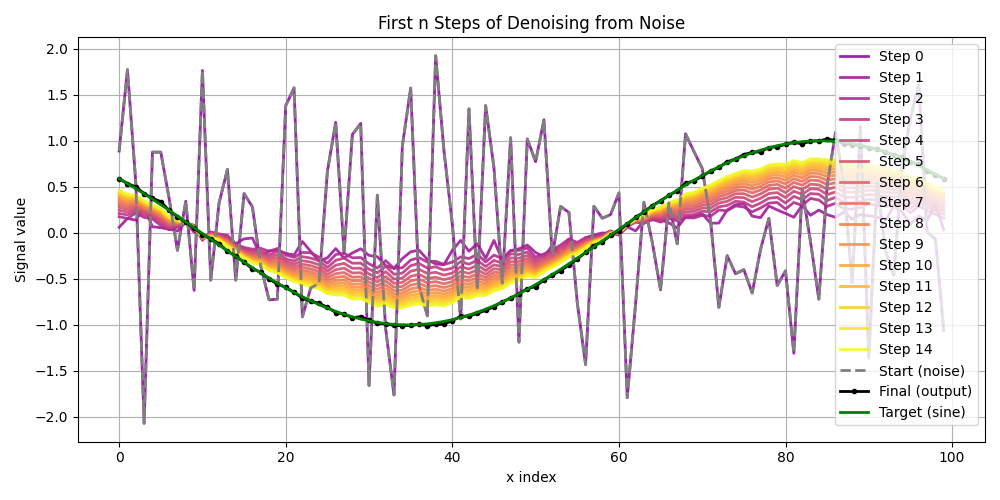
\includegraphics[width=0.9\textwidth]{images/diffusion_denoising.png}
    \caption{%
        The first 15 steps of the denoising process, starting from white noise (dashed gray).
        Colored curves represent the intermediate states.
        The model quickly adjusts toward the structure of the target sine (green),
        with the final output (black dots) nearly matching it.
    }
    \label{fig:diffusion_denoising}
\end{figure}



\subsection{A Minimal Diffusion Denoising Example}

To demonstrate the principle of diffusion models in a simple and interpretable setting, we construct a minimal 1D example: starting from white noise, a neural network learns to iteratively denoise it toward a target sine curve. We use PyTorch to define and train a small denoising network that learns this reconstruction process in a class-conditional setup.

%------------------------------------------------------------------------------
%
%------------------------------------------------------------------------------
\paragraph{Step 1: Configuration and Target Signal.} We define the sine wave classes, select one target curve, and generate the corresponding label as a one-hot vector.

\begin{codeonly}{Setup Example for Diffusion Network}
import torch
import torch.nn as nn
import torch.optim as optim
import matplotlib.pyplot as plt

# --- Config ---
n_points = 100
n_steps = 50
noise_std = 0.2
class_idx = 2  # Select sine class 0 to 4

# --- Generate sine waves ---
x = torch.linspace(0, 2 * torch.pi, n_points)
phases = torch.arange(5) * (2 * torch.pi / 5)
sine_set = torch.stack([torch.sin(x + p) for p in phases])
x_target = sine_set[class_idx].unsqueeze(0)  # shape [1, n_points]
label = torch.nn.functional.one_hot(torch.tensor([class_idx]), num_classes=5).float()
\end{codeonly}

This sets up our clean signal \( \mathbf{x}_0 \) and class information to be used throughout training and inference.

%------------------------------------------------------------------------------
%
%------------------------------------------------------------------------------
\paragraph{Step 2: Define the Denoising Network.} We now define a small MLP that takes as input the noisy signal and the class label (concatenated) and outputs a denoised signal of the same shape.

\begin{codeonly}{Network for Diffusion Inversion}
# --- Model ---
class DenoiseMLP(nn.Module):
    def __init__(self, n_points, n_classes):
        super().__init__()
        self.net = nn.Sequential(
            nn.Linear(n_points + n_classes, 128),
            nn.ReLU(),
            nn.Linear(128, 128),
            nn.ReLU(),
            nn.Linear(128, n_points)
        )
    def forward(self, x, label):
        return self.net(torch.cat([x, label], dim=1))

model = DenoiseMLP(n_points, n_classes=5)
\end{codeonly}

This architecture is deliberately small to keep training fast and interpretable. The model learns a mapping from noisy versions of the signal to cleaner versions at earlier diffusion steps.

%------------------------------------------------------------------------------
%
%------------------------------------------------------------------------------
\paragraph{Step 3: Training the Denoising Model.} The training process simulates a forward diffusion process by adding Gaussian noise to the clean signal in small increments, then teaches the model to reverse this process step by step. We use a simple mean squared error (MSE) loss to train the model to predict the less-noisy signal at the previous step.

\begin{codeonly}{Optimizer and Noise Generator}
optimizer = optim.Adam(model.parameters(), lr=1e-3)
loss_fn = nn.MSELoss()

# Add progressive noise
def add_noise_sequence(x0, n_steps, noise_std):
    x = x0.clone()
    trajectory = [x]
    for _ in range(n_steps):
        x = x + (noise_std / n_steps) * torch.randn_like(x)
        trajectory.append(x)
    return trajectory
\end{codeonly}

The function \texttt{add\_noise\_sequence} returns a list of noisy versions \( \mathbf{x}_t \) starting from the clean signal \( \mathbf{x}_0 \). Each step adds a small amount of Gaussian noise.

The training loop samples a noisy trajectory and trains the model to denoise from \( \mathbf{x}_t \) to \( \mathbf{x}_{t-1} \), starting from the noisiest point and moving backwards:

\begin{codeonly}{Diffusion Network Training Loop}
for epoch in range(1001):
    noisy_traj = add_noise_sequence(x_target, n_steps, noise_std)
    loss = 0.0
    for t in reversed(range(1, len(noisy_traj))):
        x_in = noisy_traj[t]
        x_out = noisy_traj[t-1]
        x_pred = model(x_in, label)
        loss += loss_fn(x_pred, x_out)
    loss /= n_steps
    optimizer.zero_grad()
    loss.backward()
    optimizer.step()
    if epoch % 100 == 0:
        print(f"Epoch {epoch}: Loss = {loss.item():.6f}")
\end{codeonly}

The model is trained on one fixed sine class, identified by its one-hot label. The loss accumulates over all denoising steps and is averaged before each optimization step. This process teaches the model to reverse the noisy trajectory — one step at a time — and eventually generate a clean sine signal when starting from white noise.

%------------------------------------------------------------------------------
%
%------------------------------------------------------------------------------
\paragraph{Step 4: Reverse Sampling and Visualization}

After training, we use the model as an iterative denoiser: starting from white noise, we repeatedly apply the learned function to reduce noise and guide the signal toward a sine-like structure. This mimics the reverse trajectory of a diffusion process.

\begin{codeonly}{Denoise from White Noise}
# --- Reverse from noise ---
with torch.no_grad():
    x = torch.randn_like(x_target)
    x_start = x.clone()
    traj = [x.squeeze().numpy()]
    for _ in range(n_steps):
        x = model(x, label)
        traj.append(x.squeeze().numpy())
\end{codeonly}

The variable \texttt{traj} stores each intermediate signal. To observe how the denoising unfolds, we visualize the first few steps of the reconstruction process.

\begin{codeonly}{}
# --- Plot first 15 steps + start, final, target ---
import numpy as np
plt.figure(figsize=(10, 5))

steps_to_plot = list(range(0, 15))  # show early progress
colors = plt.cm.plasma(np.linspace(0.3, 1.0, len(steps_to_plot)))

for i, t in enumerate(steps_to_plot):
    plt.plot(traj[t], color=colors[i], alpha=0.9, linewidth=2, label=f"Step {t}")

# Add clearly labeled curves
plt.plot(x_start.squeeze().numpy(), 'gray', linestyle='dashed', linewidth=2, label="Start (noise)")
plt.plot(traj[-1], 'k.', linestyle='-', linewidth=2, label="Final (output)")
plt.plot(x_target.squeeze().numpy(), 'g', linestyle='-', linewidth=2, label="Target (sine)")

plt.title("First n Steps of Denoising from Noise")
plt.xlabel("x index")
plt.ylabel("Signal value")
plt.legend(loc="upper right")
plt.grid(True)
plt.tight_layout()
plt.savefig("diffusion_denoising.png")
plt.show()
\end{codeonly}

The resulting figure (see Figure~\ref{fig:diffusion_denoising}) shows the progressive alignment of the noisy signal toward the clean sine curve.

%------------------------------------------------------------------------------
%
%------------------------------------------------------------------------------
\subsection{Generating Functions from White Noise Using Conditional Diffusion}

In many physical systems, outputs are structured signals — for example, 1D fields like temperature profiles or time-series measurements. These are influenced by both stochastic variability and contextual constraints (e.g., location, boundary conditions, or categories). 

In this section, we explore how diffusion models can generate such signals starting from white noise and guided by a conditioning input — here, a class index that selects one of several sine wave types. This basic idea generalizes to more complex applications, such as generating spatial weather fields from forecasts or even from text prompts.

%------------------------------------------------------------------------------
\subsubsection*{Target Functions: Shifted Sine Waves}

We define \( n_\text{classes} \) shifted sine curves:
\[
s_k(x) = \sin\left(x + \frac{2\pi k}{n_\text{classes}}\right), \quad k = 0, \dots, n_\text{classes} - 1,
\]
sampled on a fixed grid. Each class represents a different target signal.

%------------------------------------------------------------------------------
\subsubsection*{Training the Reverse Process}

The model is trained to denoise progressively. We begin from a clean sine wave \( x_0 \), add noise step-by-step to generate a trajectory \( x_0, x_1, ..., x_T \), and train the model to learn the reverse steps.

Each step of the model takes a noisy signal \( x_t \) and a one-hot encoded class label \( \mathbf{y} \), and predicts the cleaner \( x_{t-1} \). The total loss accumulates the mean squared error across all reverse steps:

\begin{codeonly}{training loop with class-conditioned denoising}
optimizer = optim.Adam(model.parameters(), lr=0.001)
mse_loss = nn.MSELoss()

for epoch in range(601):
    idx = torch.randint(0, n_classes, (batch_size,))
    x_clean = sine_set[idx]
    labels = torch.nn.functional.one_hot(idx, num_classes=n_classes).float()

    x_t = x_clean.clone()
    trajectory = [x_t.clone()]
    for _ in range(n_steps):
        x_t = add_noise_step(x_t, noise_std / n_steps)
        trajectory.append(x_t.clone())

    loss = 0.0
    for step in reversed(range(1, n_steps + 1)):
        x_input = trajectory[step]
        x_target = trajectory[step - 1]
        x_input_with_label = torch.cat([x_input, labels], dim=1)
        x_pred = model(x_input_with_label)

        loss_denoise = mse_loss(x_pred, x_target)
        target_template = labels @ sine_set
        loss_template = mse_loss(x_pred, target_template)
        cos = nn.CosineSimilarity(dim=1)
        loss_cos = 1 - cos(x_pred, target_template).mean()
        loss_align = mse_loss(x_pred, x_clean) if step == 1 else 0.0

        loss += loss_denoise + 2 * loss_template + 0.2 * loss_cos

    loss /= n_steps
    optimizer.zero_grad()
    loss.backward()
    optimizer.step()
\end{codeonly}

%------------------------------------------------------------------------------
\subsubsection*{Generating a Function from Noise}

After training, we can generate a signal starting from white noise. The only input to the model is a class label — for example, the instruction ``give me the curve for class 2.'' The model then iteratively denoises the signal.

\begin{codeonly}{sampling one function from white noise}
x = torch.randn(1, n_points)
label = torch.nn.functional.one_hot(torch.tensor([class_idx]), num_classes=n_classes).float()

for _ in range(n_steps):
    x_input = torch.cat([x, label], dim=1)
    x = amplify * model(x_input)
\end{codeonly}

%------------------------------------------------------------------------------
\subsubsection*{Visualization and Results}

Figure~\ref{fig:sample-overlay} shows multiple generated functions for different class labels, compared to the reference sine curves. Despite starting from pure noise, the output converges to class-consistent functions.

\begin{figure}[h]
\centering
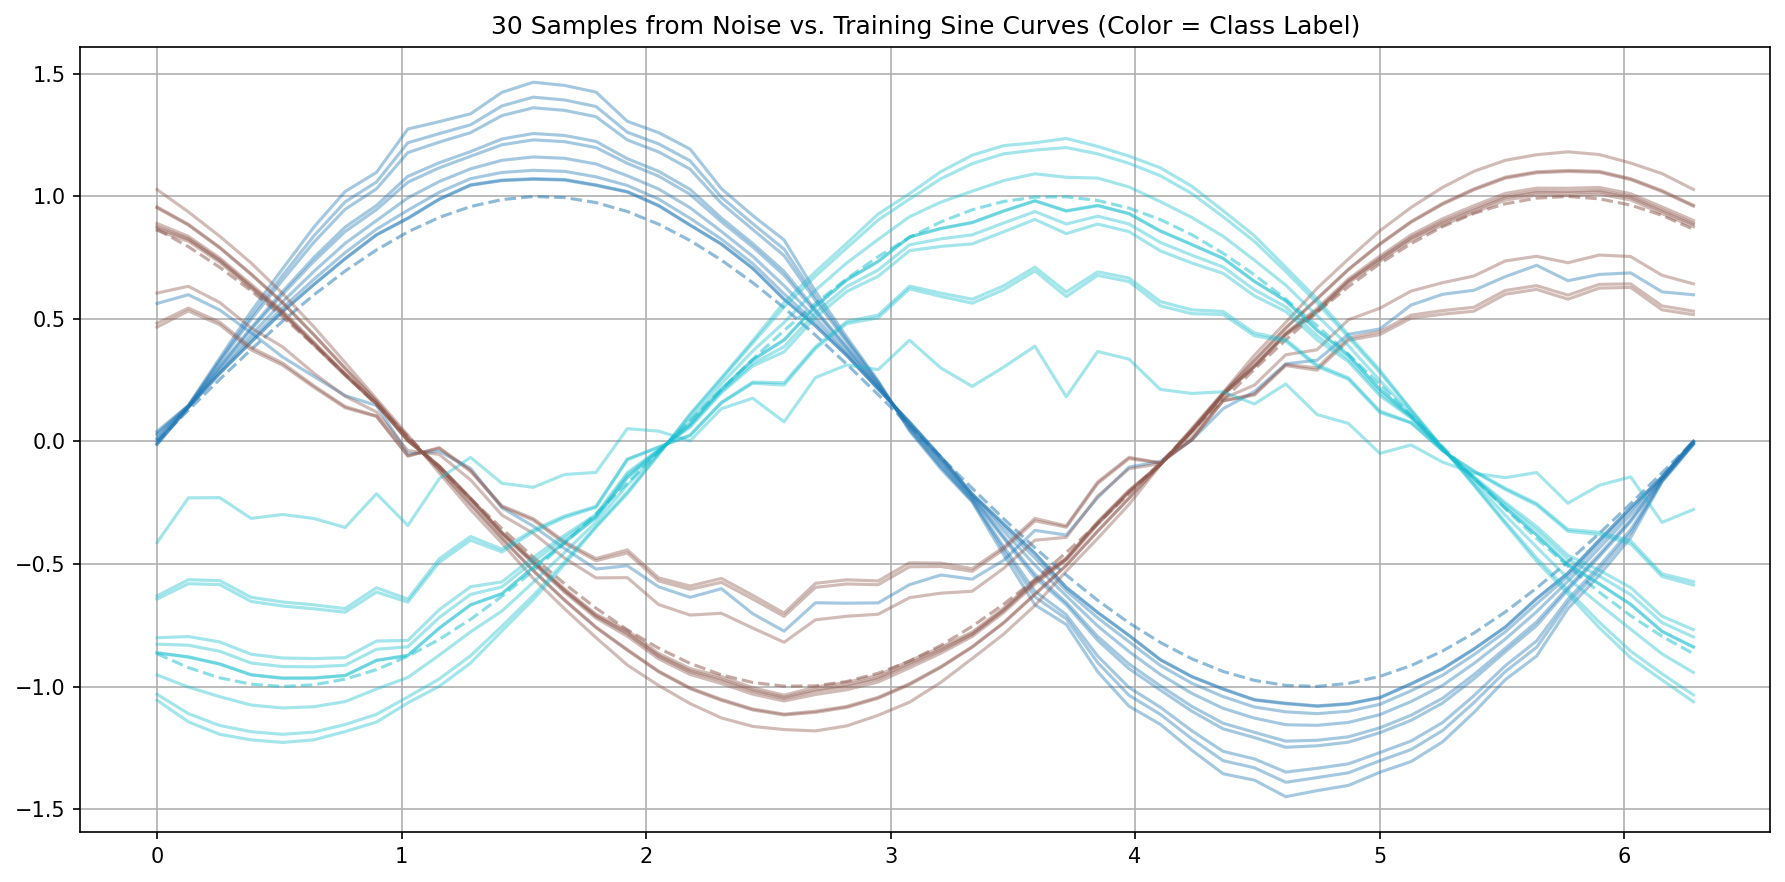
\includegraphics[width=\textwidth]{images/samples_vs_sines_conditioned.png}
\caption{Samples generated from white noise and guided by class label. Colored lines show generated samples, dashed lines the target sine functions.}
\label{fig:sample-overlay}
\end{figure}

To visualize how structure emerges, we also track full denoising trajectories. In each subplot of Figure~\ref{fig:step-by-step}, the signal starts as noise and evolves step-by-step toward the final shape. The gray curve is the ground-truth sine.

\begin{figure}[h]
\centering
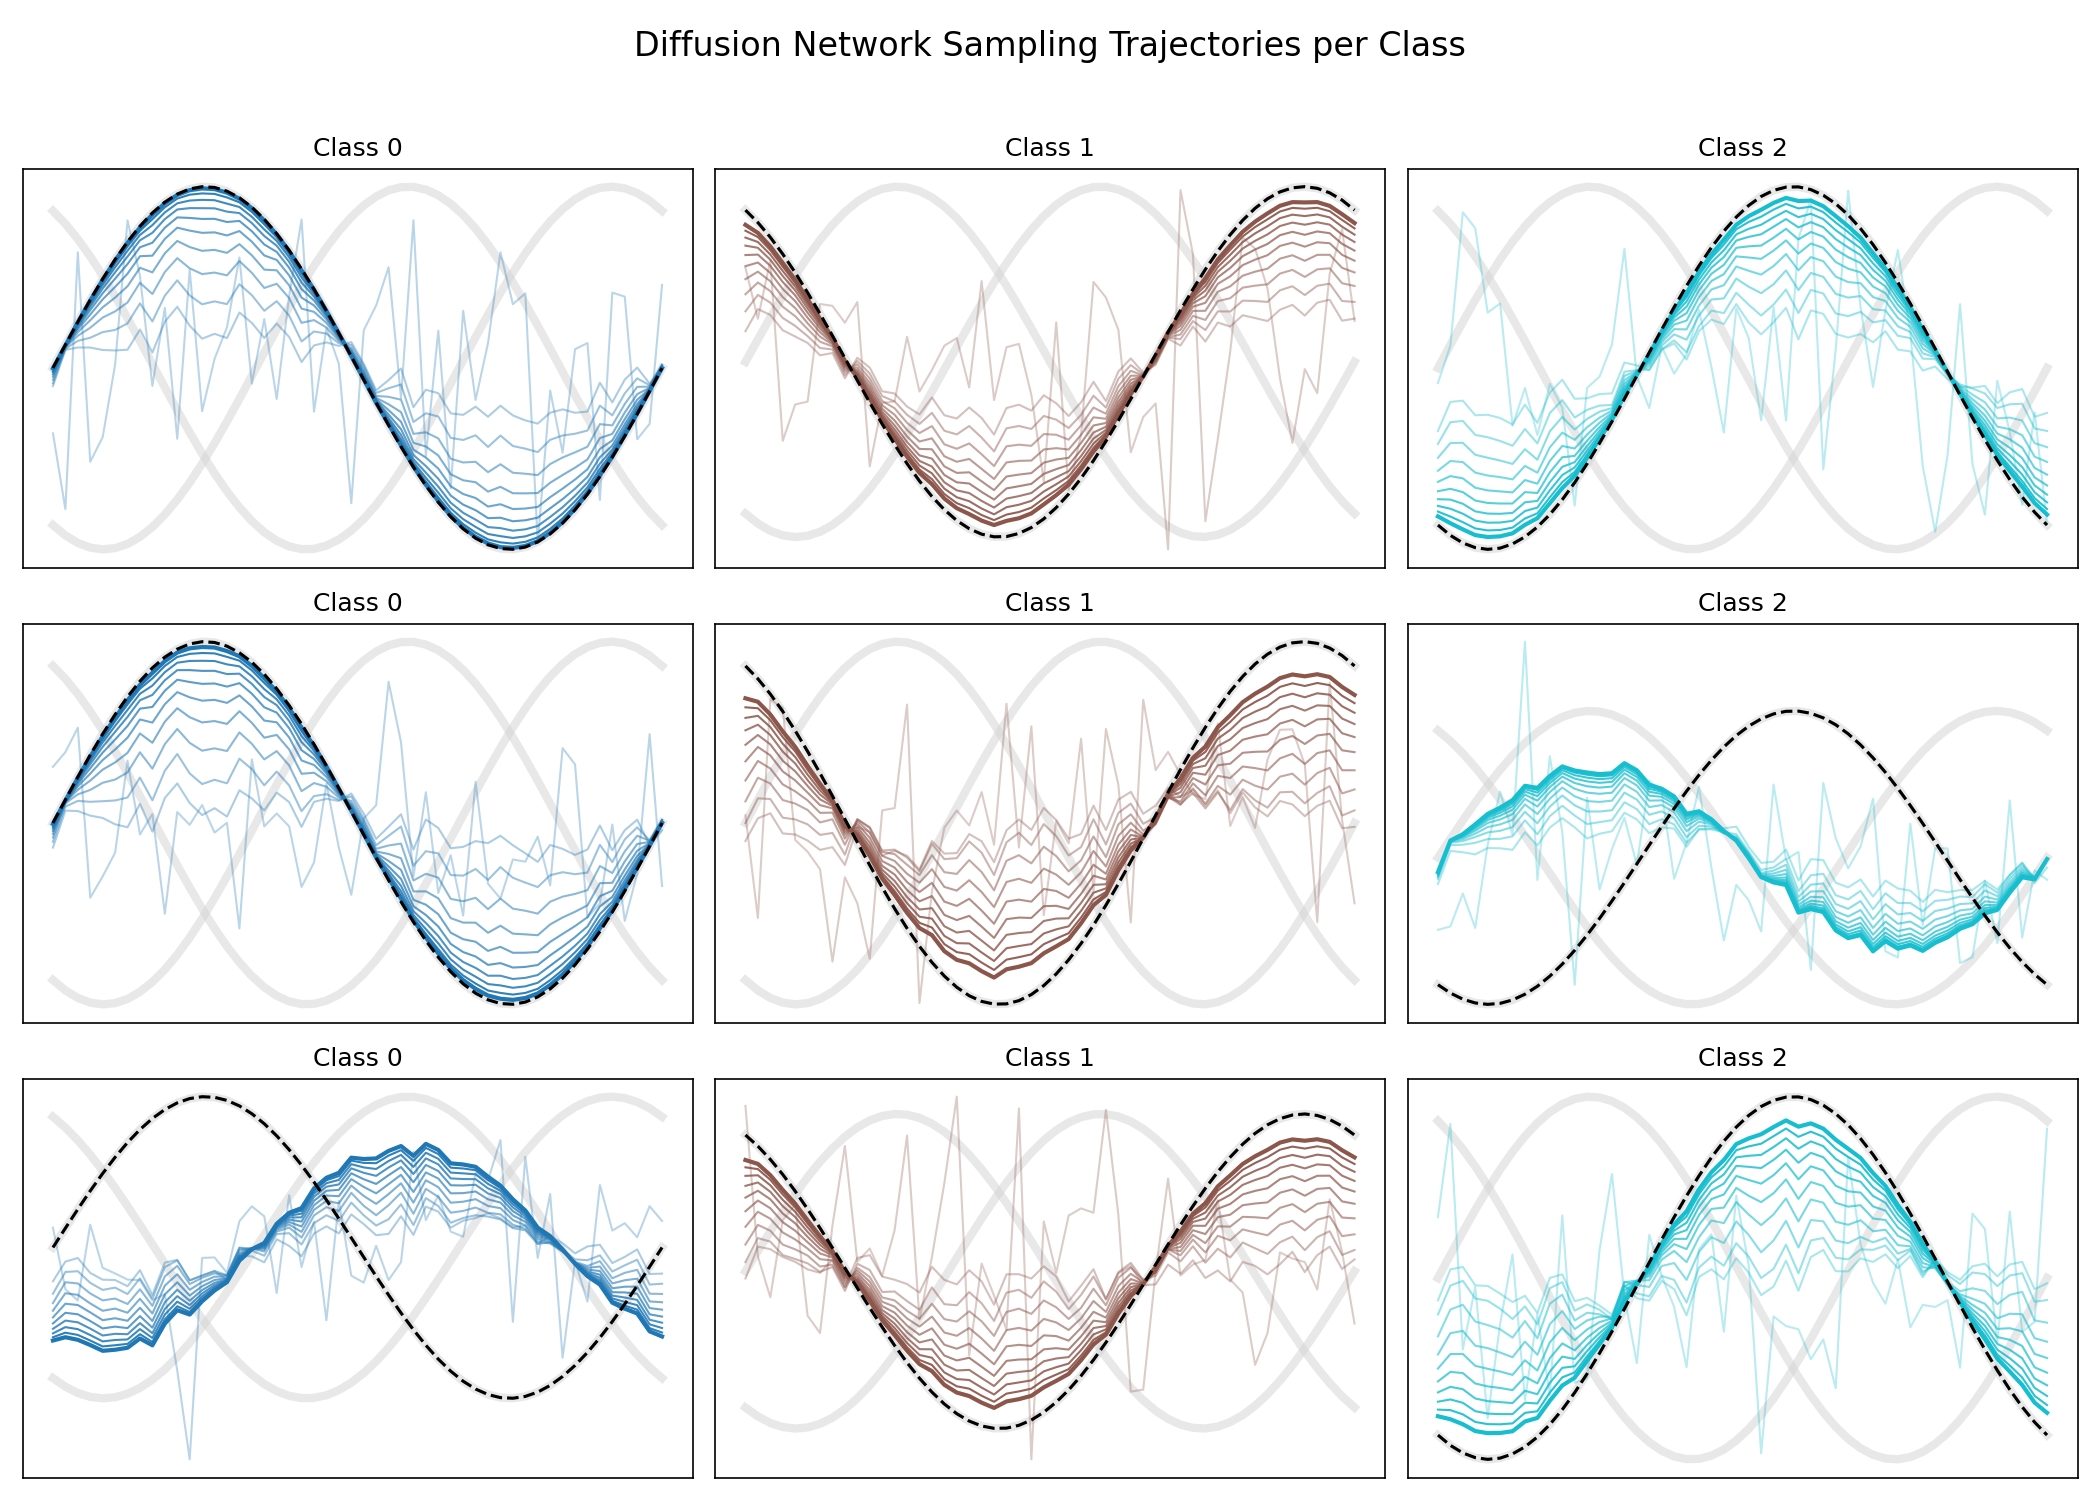
\includegraphics[width=\textwidth]{images/diffusion_network_sampling.png}
\caption{Denoising trajectories for 9 generated signals. Each panel shows 10 intermediate steps from noise to final output. The gray curve is the class target.}
\label{fig:step-by-step}
\end{figure}

%------------------------------------------------------------------------------
\subsubsection*{Summary and Perspective}

This example illustrates the core idea of diffusion-based generation: from noise to signal, guided by side information. While we use class labels here, the conditioning input could be general — spatial context, metadata, or even a short natural language prompt.

In weather and climate modeling, this approach can be extended to:
\begin{itemize}
    \item Generate ensemble forecast members from coarse NWP input,
    \item Downscale global simulations to local weather fields,
    \item Impute missing or corrupted observations,
    \item Build hybrid models integrating physics and data.
\end{itemize}

We now have a powerful framework to model structured distributions over functions — not by directly learning the output, but by learning how to refine noise into data.

%------------------------------------------------------------------------------
%
%------------------------------------------------------------------------------
\subsection{Why it Works: Diffusion Network Theory for the Scalar Case}

To better understand the probabilistic nature of diffusion models, we consider a one-dimensional (scalar) example. Let the original data distribution be a Gaussian:
\[
x_0 \sim \mathcal{N}(\mu_0, \sigma_0^2),
\]
with a concrete choice of parameters \( \mu_0 = 3 \), \( \sigma_0^2 = 1 \). The forward diffusion step adds Gaussian noise:
\[
x_1 = x_0 + \epsilon, \quad \epsilon \sim \mathcal{N}(0, \sigma^2).
\]
By basic facts on Gaussian distributions, the distribution of \( x_1 \) becomes:
\[
x_1 \sim \mathcal{N}(\mu_0, \sigma_0^2 + \sigma^2).
\]

%------------------------------------------------------------------------------
\paragraph{Optimal Denoiser.}
The optimal denoiser in the mean-squared error sense is the conditional expectation:
\[
f^*(x_1) := \mathbb{E}[x_0 \mid x_1].
\]
Lets do the little derivation here. Assume \( x_0 \sim \mathcal{N}(\mu_0, \sigma_0^2) \) is the clean signal, and the observed noisy signal is \( x_1 = x_0 + \epsilon \), where \( \epsilon \sim \mathcal{N}(0, \sigma^2) \) is independent Gaussian noise. Then, using Bayes' theorem, the posterior distribution of \( x_0 \) given \( x_1 \) is:
\[
p(x_0 \mid x_1) = \frac{p(x_1 \mid x_0) \cdot p(x_0)}{p(x_1)}.
\]
Let us recall a standard identity for univariate Gaussian distributions, noting that $p(x_1)$ serves as normalization constant in the Bayes formula. The (unnormalized) product of two Gaussians 
\[
\mathcal{N}(x \mid \mu_1, \sigma_1^2) \cdot \mathcal{N}(x \mid \mu_2, \sigma_2^2) 
\propto \mathcal{N}\left(x \mid \mu_{\times}, \sigma_{\times}^2\right),
\]
is again a Gaussian with:
\begin{align*}
\sigma_{\times}^2 &= \left( \frac{1}{\sigma_1^2} + \frac{1}{\sigma_2^2} \right)^{-1}
= \frac{\sigma_1^2 \sigma_2^2}{\sigma_1^2 + \sigma_2^2}, \\
\mu_{\times} &= \sigma_{\times}^2 \left( \frac{\mu_1}{\sigma_1^2} + \frac{\mu_2}{\sigma_2^2} \right)
= \frac{\sigma_2^2 \mu_1 + \sigma_1^2 \mu_2}{\sigma_1^2 + \sigma_2^2}.
\end{align*}
We now apply this directly to the posterior:
\[
p(x_0 \mid x_1) \propto p(x_1 \mid x_0) \cdot p(x_0),
\]
with:
\[
p(x_0) = \mathcal{N}(x_0 \mid \mu_0, \sigma_0^2), \qquad
p(x_1 \mid x_0) = \mathcal{N}(x_1 \mid x_0, \sigma^2),
\]
which we can rewrite as:
\[
p(x_1 \mid x_0) = \mathcal{N}(x_0 \mid x_1, \sigma^2),
\]
so the product becomes:
\[
p(x_0 \mid x_1) \propto \mathcal{N}(x_0 \mid \mu_0, \sigma_0^2) \cdot \mathcal{N}(x_0 \mid x_1, \sigma^2).
\]
By the above rule, the posterior is again Gaussian:
\[
p(x_0 \mid x_1) = \mathcal{N}(x_0 \mid \mu_{\text{post}}, \sigma_{\text{post}}^2),
\]
with:
\begin{align*}
\sigma_{\text{post}}^2 &= \frac{\sigma_0^2 \cdot \sigma^2}{\sigma_0^2 + \sigma^2}, \\
\mu_{\text{post}} &= \frac{\sigma^2 \mu_0 + \sigma_0^2 x_1}{\sigma_0^2 + \sigma^2}.
\end{align*}
This means
\begin{equation}
f^*(x_1) = \mathbb{E}[x_0 \mid x_1] = \mu_{\text{post}} = \frac{\sigma^2 \mu_0 + \sigma_0^2 x_1}{\sigma_0^2 + \sigma^2}
= x_1 + (\mu_0 - x_1 )\cdot \frac{\sigma^2}{\sigma_0^2 + \sigma^2}.
\label{opt estimator}
\end{equation}
Hence, the optimal denoiser is a linear function pulling \( x_1 \) toward \( \mu_0 \), and reducing the variance.  
Using 
\[
\mathrm{Var}(aX+b) = a^2 \cdot Var(X)
\]
the variance of \( f^*(x_1) \) in dependence of $x_1$ is calculated by:
\[
\mathrm{Var}(f^*(x_1)) = \left( \frac{\sigma_0^2}{\sigma_0^2 + \sigma^2} \right)^2 \cdot \mathrm{Var}(x_1) = \frac{\sigma_0^4}{\sigma_0^2 + \sigma^2}.
\]
To recover the original distribution, we must sample from the full posterior:
\[
x_0 = f^*(x_1) + \sqrt{\sigma_{\text{post}}^2} \cdot \xi, \quad \xi \sim \mathcal{N}(0, 1).
\]
Then, the total variance becomes:
\[
\mathrm{Var}(x_0) = \mathrm{Var}(f^*(x_1)) + \sigma_{\text{post}}^2
= \frac{\sigma_0^4 + \sigma_0^2 \cdot \sigma^2}{\sigma_0^2 + \sigma^2}
= \frac{\sigma_0^2 (\sigma_0^2 + \sigma^2)}{\sigma_0^2 + \sigma^2}
= \sigma_0^2.
\]

%------------------------------------------------------------------------------
\paragraph{Why Iterative Sampling is Necessary.}
A single denoising step, modeled as the conditional expectation \( f^*(x_1) = \mathbb{E}[x_0 \mid x_1] \), does not recover the original mean \( \mu_0 \) of the data distribution. Instead, it produces a posterior mean \( \mu_{\text{post}} \) that is a weighted combination of \( x_1 \) and \( \mu_0 \). The output is therefore still biased by the noise in \( x_1 \).

To progressively move towards the original distribution \( \mathcal{N}(\mu_0, \sigma_0^2) \), multiple denoising steps are needed. Each step slightly reduces the noise and shifts the estimate closer to the clean data manifold. This is the essence of iterative sampling in diffusion models: a sequence of reverse transitions from noise to data.

Suppose we add Gaussian noise in \( n \) steps, where each step adds noise with standard deviation \( \sigma / n \). The variance of the noise added in step \( k \) is thus \( \sigma_k^2 = \sigma^2 / n^2 \), and the total noise variance after all \( n \) steps is:
\[
\sigma_{\text{total}}^2 = \sum_{k=1}^n \frac{\sigma^2}{n^2} = \frac{\sigma^2}{n}.
\]
Let \( x_n \) denote the final noisy sample. To denoise step-by-step, we apply the optimal estimator in reverse order, using the posterior mean:
\[
\mathbb{E}[x_{k-1} \mid x_k] = (1 - \gamma_k) x_k + \gamma_k \mu^{(prior)}_{k-1},
\]
where
\[
\gamma_k
= \frac{\frac{\sigma^2}{n^2}}{\sigma_0^2 + \frac{(k-1)\sigma^2}{n^2} + \frac{\sigma^2}{n^2}}
= \frac{\sigma^2}{{n^2 \sigma_0^2} + k \sigma^2}.
\]
and \( \mu^{(prior)}_{k-1} \) is the expected prior mean of \( x_{k-1} \) before seeing $x_k$, obtained from previous steps, such as $\mu_0$ if we did not rescale our original signal or the rescaled values when rescaling is used. This defines a recursion:
\[
x_{k-1} = (1 - \gamma_k) x_k + \gamma_k \mu_0 = x_k + \gamma_k ( \mu_0 - x_k),
\]
starting from \( x_n \). Since $\gamma_k$ is consistently larger than 
\[
\gamma_{min} := \frac{\sigma^2}{n^2 \sigma_0^2 + n \sigma^2}, 
\] 
unrolling this recursion 
\[
x_{k-1} = (1 - \gamma_{\min}) x_k + \gamma_{\min} \mu_0
\]
for \( k = n, n-1, \dotsc, 1 \), with fixed \( \gamma_{\min} \in (0, 1) \), we obtain (based the standard geometric series argument)
\[
x_0 = (1 - \gamma_{\min})^n x_n + \left(1 - (1 - \gamma_{\min})^n \right) \mu_0
\rightarrow \mu_0, \;\; n \rightarrow \infty, 
\]
i.e.\ it shows that the denoising path progressively pulls the expectation back toward the original mean $\mu_0$. Thus, iterative denoising converges to the true mean in the limit of infinitely many small noise-injection and denoising steps.

This confirms that iterative denoising with many small steps recovers the original distribution mean — even though each individual step is only a small correction.

%------------------------------------------------------------------------------
\paragraph{Conclusion.} This simple scalar example demonstrates a crucial aspect of diffusion models:
\begin{itemize}
    \item The optimal denoiser \( f^*(x_k) \) estimates the \emph{mean} of the reverse distribution.
    \item To match the original data distribution, one must \emph{sample} from the full posterior, which includes adding back calibrated noise.
    \item This justifies the stochastic reverse process used in diffusion models, where noise is injected in each denoising step.
\end{itemize}

%==============================================================================
% 
%==============================================================================
\section{Flexible Graph Networks for Learning from Sparse Observations}

\subsection{A Naive Approach: Learning Functions from Sparse Observations}

In this first implementation, we train a Graph Neural Network (GNN) to reconstruct simple functions (sine and cosine) from partial observations on a one-dimensional grid. The setup is intentionally minimal and includes all components required to construct, train, and apply a graph-based model. Later sections will analyze and generalize this setup.

\paragraph{Overview:}
We aim to learn a mapping from sparse observations to a full function profile by training on synthetically generated sine and cosine functions with random phases. Observations are available at every $M$-th grid point. The GNN uses a fixed neighborhood structure defined by $K$-nearest neighbors.

\vspace{1em}
\noindent The complete workflow includes the following components:

\begin{itemize}
  \item Creating the spatial grid.
  \item Defining the graph connectivity.
  \item Designing the GNN architecture.
  \item Training the model on sampled functions.
  \item Testing the model on larger and more complex domains.
\end{itemize}

\begin{figure}[ht]
  \centering
  \begin{tabular}{ccc}
    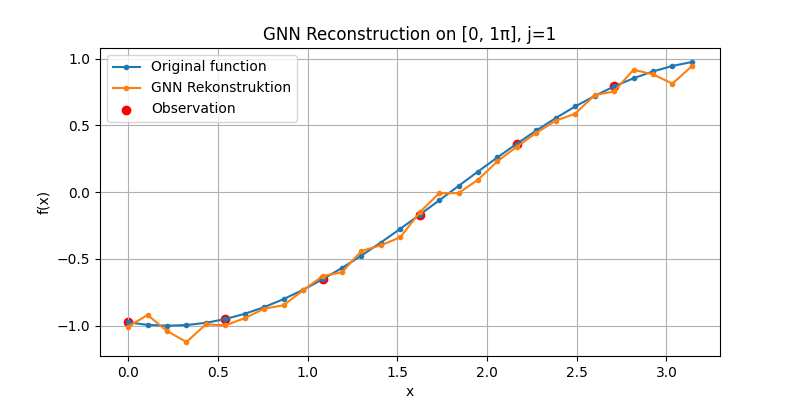
\includegraphics[width=0.3\textwidth]{images/gnn_obs_naive_j1_jj1_0.png} &
    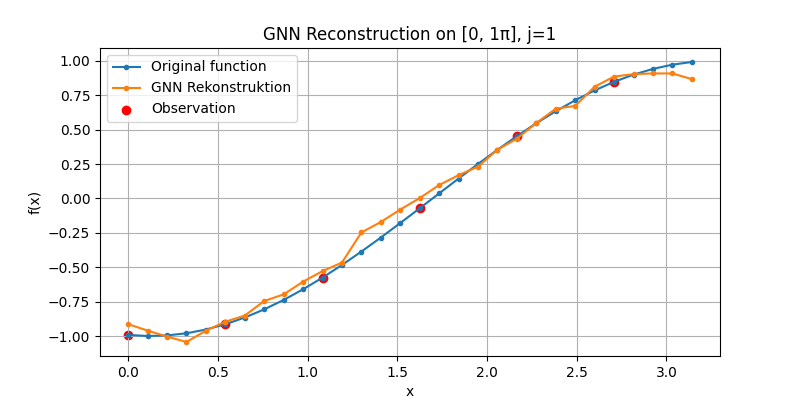
\includegraphics[width=0.3\textwidth]{images/gnn_obs_naive_j1_jj1_1.png} &
    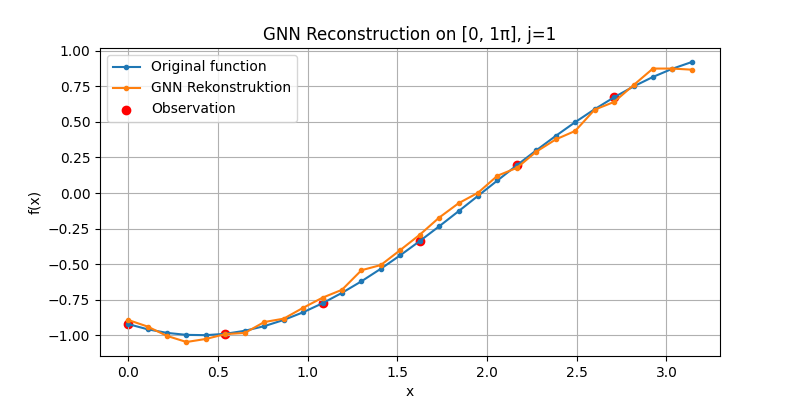
\includegraphics[width=0.3\textwidth]{images/gnn_obs_naive_j1_jj1_2.png} \\
    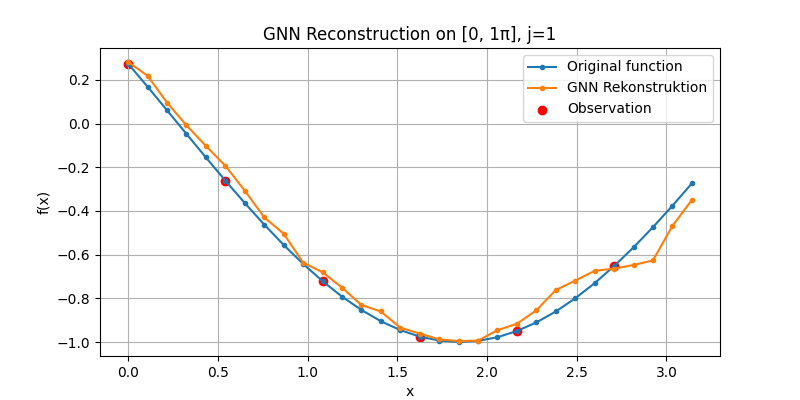
\includegraphics[width=0.3\textwidth]{images/gnn_obs_naive_j1_jj1_3.png} &
    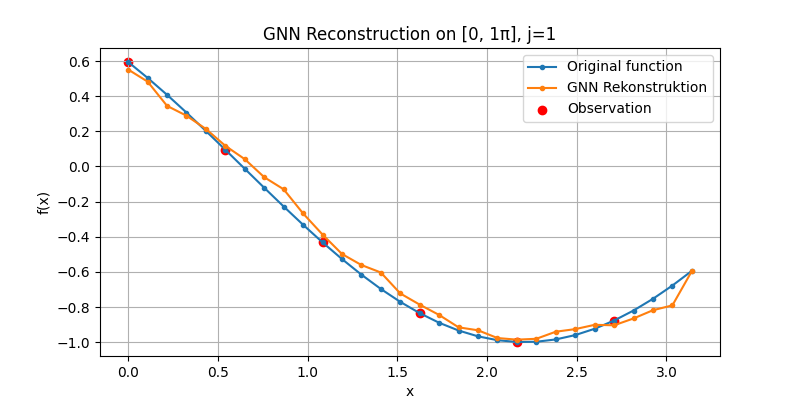
\includegraphics[width=0.3\textwidth]{images/gnn_obs_naive_j1_jj1_4.png} &
    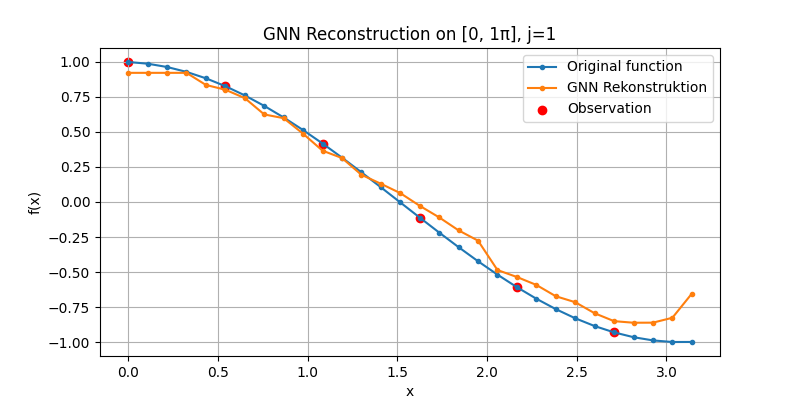
\includegraphics[width=0.3\textwidth]{images/gnn_obs_naive_j1_jj1_5.png} \\
    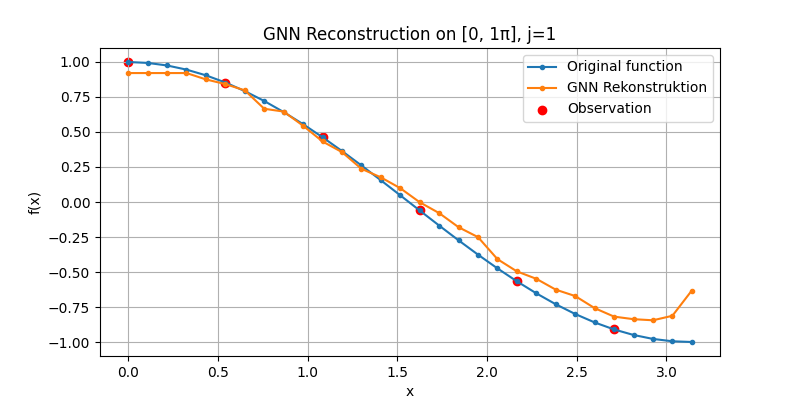
\includegraphics[width=0.3\textwidth]{images/gnn_obs_naive_j1_jj1_6.png} &
    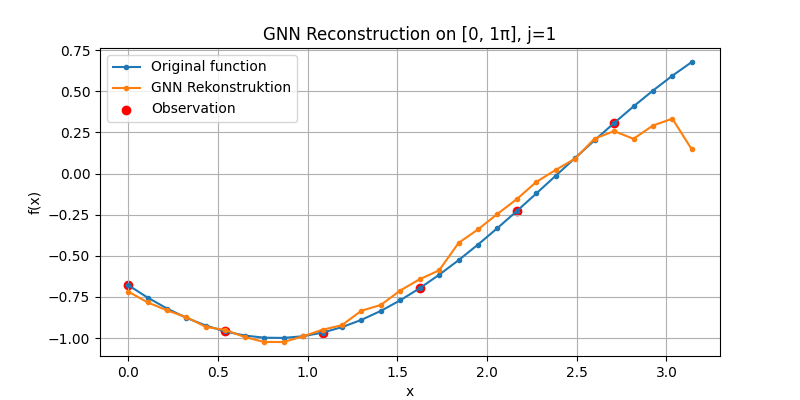
\includegraphics[width=0.3\textwidth]{images/gnn_obs_naive_j1_jj1_7.png} &
    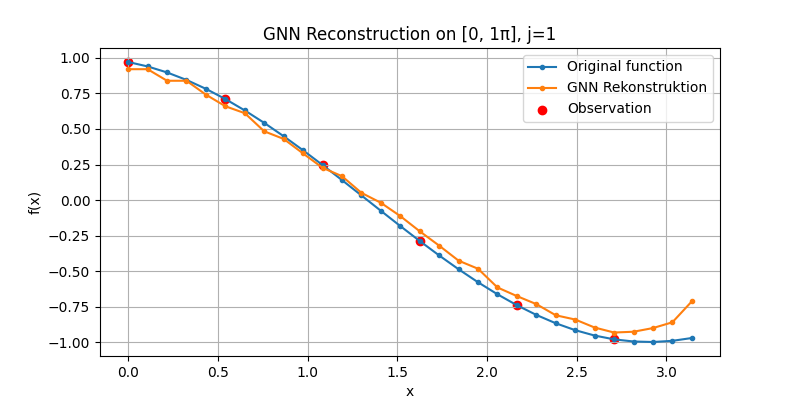
\includegraphics[width=0.3\textwidth]{images/gnn_obs_naive_j1_jj1_8.png} \\
  \end{tabular}
  \caption{GNN reconstructions for $f(x) = \cos(x + \phi)$ on $[0, \pi]$ with different phases. Each panel shows the original function, sparse observations, and the GNN prediction.}
  \label{fig:gnn_j1_jj1}
\end{figure}


\paragraph{Step 1: Libraries and Parameter Setup}

\begin{codeonly}{Imports and Parameters}
import torch
import torch.nn as nn
import torch.nn.functional as F
import numpy as np
import matplotlib.pyplot as plt

N = 30           # Number of grid points
M = 5            # Every M-th point is observed
K = 3            # Number of neighbors per node
num_epochs = 201
num_samples = 200
lr = 0.01

x_grid = torch.linspace(0, np.pi, N)
\end{codeonly}

\paragraph{Step 2: Graph Construction}

Each node is connected to itself and its $K$ neighbors on both sides. This creates a fixed undirected graph.

\begin{codeonly}{Graph Construction}
edges = []
for i in range(N):
    edges.append((i, i))  # Self-loop
    for k in range(1, K + 1):
        if i - k >= 0:
            edges.append((i, i - k))
        if i + k < N:
            edges.append((i, i + k))
edge_index = torch.tensor(edges).T  # [2, num_edges]
\end{codeonly}

\paragraph{Step 3: Model Architecture}

We define a basic GNN architecture with two message-passing layers. Each layer aggregates features from neighboring nodes and applies a linear transformation.

\begin{codeonly}{Model Definition}
class GNNLayer(nn.Module):
    def __init__(self, dim):
        super().__init__()
        self.self_lin = nn.Linear(dim, dim)
        self.neigh_lin = nn.Linear(dim, dim)

    def forward(self, x, edge_index):
        row, col = edge_index
        agg = torch.zeros_like(x)
        agg.index_add_(0, row, x[col])
        return F.relu(self.self_lin(x) + self.neigh_lin(agg))

class GNN(nn.Module):
    def __init__(self, in_dim=3, hidden=64):
        super().__init__()
        self.input_proj = nn.Linear(in_dim, hidden)
        self.gnn1 = GNNLayer(hidden)
        self.gnn2 = GNNLayer(hidden)
        self.out = nn.Linear(hidden, 1)

    def forward(self, x, edge_index):
        x = F.relu(self.input_proj(x))
        x = self.gnn1(x, edge_index)
        x = self.gnn2(x, edge_index)
        return self.out(x).squeeze(-1)

model = GNN(in_dim=3)
opt = torch.optim.Adam(model.parameters(), lr=lr)
\end{codeonly}

\begin{figure}[ht]
  \centering
  \begin{tabular}{cccc}
    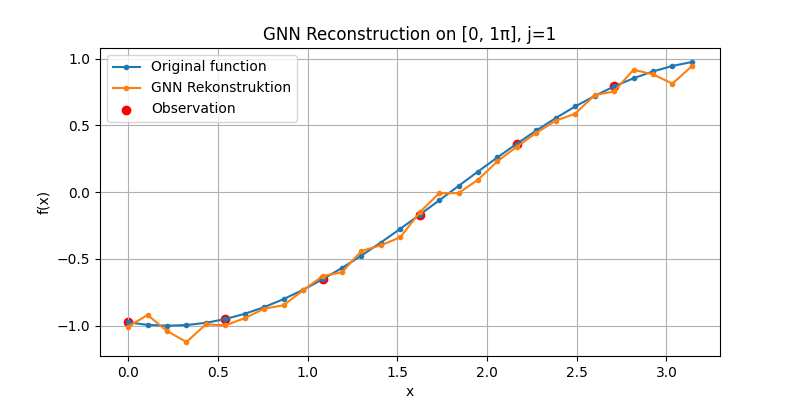
\includegraphics[width=0.23\textwidth]{images/gnn_obs_naive_j1_jj1_0.png} &
    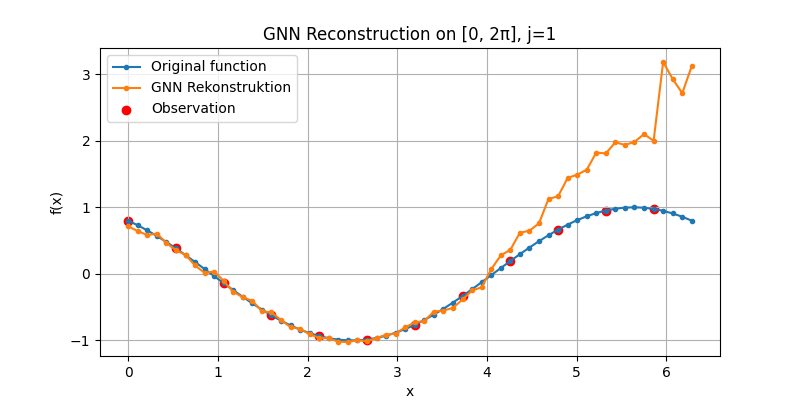
\includegraphics[width=0.23\textwidth]{images/gnn_obs_naive_j1_jj2_0.png} &
    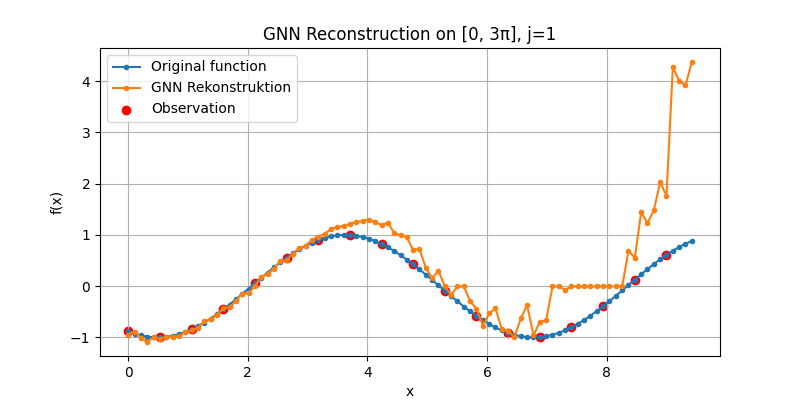
\includegraphics[width=0.23\textwidth]{images/gnn_obs_naive_j1_jj3_0.png} &
    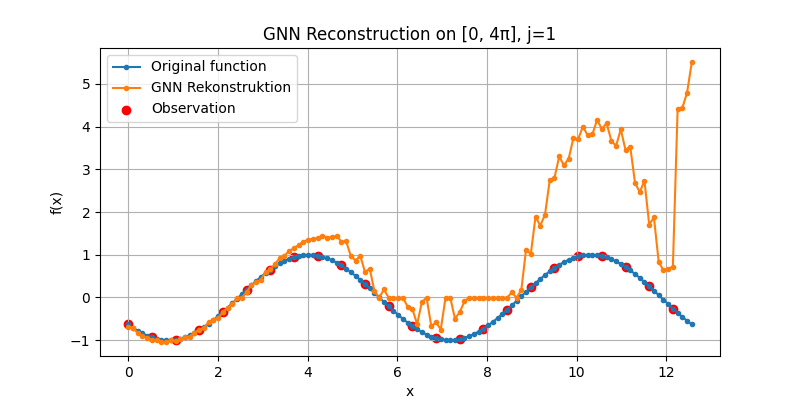
\includegraphics[width=0.23\textwidth]{images/gnn_obs_naive_j1_jj4_0.png} \\
    $\texttt{j=1, jj=1}$ & $\texttt{j=1, jj=2}$ & $\texttt{j=1, jj=3}$ & $\texttt{j=1, jj=4}$ \\
  \end{tabular}
  \caption{Generalization of the GNN to longer intervals. All test functions use $f(x) = \cos(x + \phi)$ but are evaluated on increasing domains $[0, jj \cdot \pi]$ with $jj = 1, 2, 3, 4$. The model was trained only on $[0, \pi]$.}
  \label{fig:gnn_generalization_jj}
\end{figure}


\paragraph{Step 4: Training Loop}

The model is trained to reconstruct either a sine or cosine function with random phase. Observations are only available at every $M$-th grid point. The input to each node includes the position $x$, the (masked) observation value, and a binary mask.

\begin{codeonly}{Training Loop}
for epoch in range(num_epochs):
    losses = []
    for _ in range(num_samples):
        phase = torch.rand(1).item() * np.pi
        f_type = torch.randint(0, 2, (1,)).item()
        f = lambda x: torch.sin(x + phase) if f_type == 0 else torch.cos(x + phase)
        y_true = f(x_grid)

        mask = torch.zeros(N)
        mask[::M] = 1.0
        obs_y = y_true * mask

        x_feat = torch.stack([x_grid, obs_y, mask], dim=1)

        model.train()
        pred = model(x_feat, edge_index)
        loss = F.mse_loss(pred, y_true)
        opt.zero_grad()
        loss.backward()
        opt.step()
        losses.append(loss.item())

    if epoch % 50 == 0:
        print(f"Epoch {epoch}: Loss = {np.mean(losses):.6f}")
\end{codeonly}

\begin{figure}[ht]
  \centering
  \begin{tabular}{cccc}
    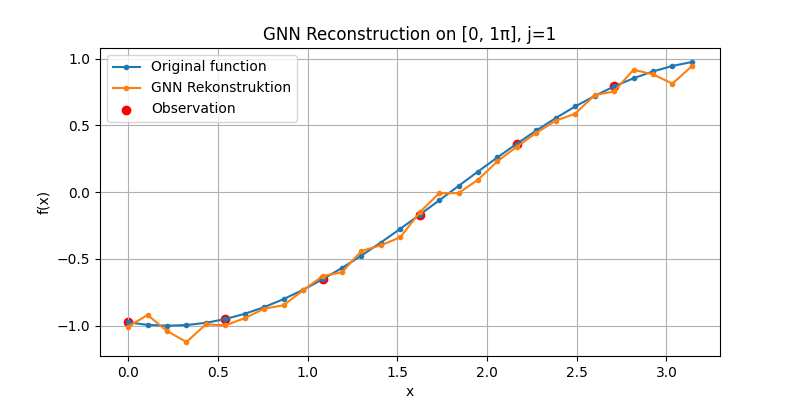
\includegraphics[width=0.23\textwidth]{images/gnn_obs_naive_j1_jj1_0.png} &
    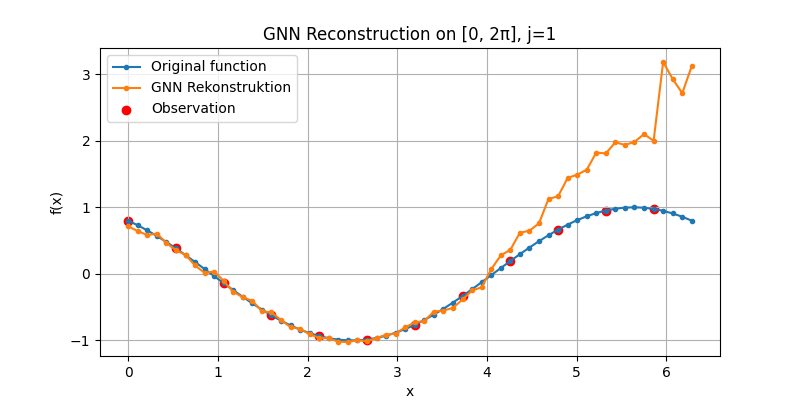
\includegraphics[width=0.23\textwidth]{images/gnn_obs_naive_j1_jj2_0.png} &
    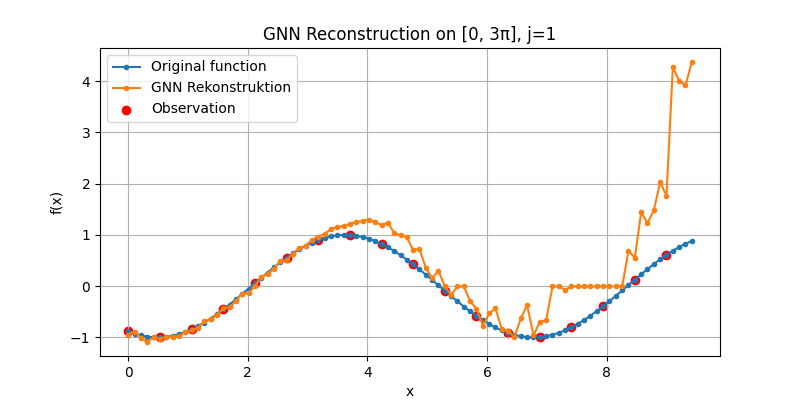
\includegraphics[width=0.23\textwidth]{images/gnn_obs_naive_j1_jj3_0.png} &
    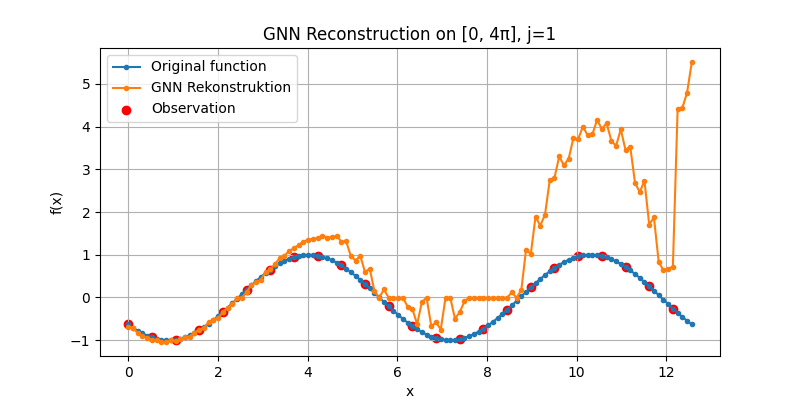
\includegraphics[width=0.23\textwidth]{images/gnn_obs_naive_j1_jj4_0.png} \\
    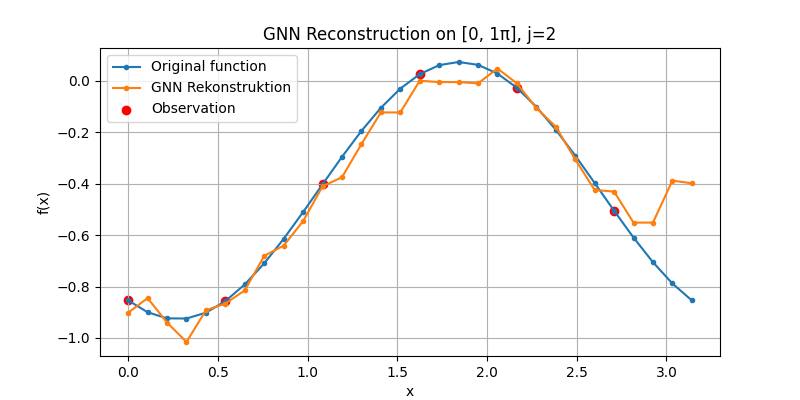
\includegraphics[width=0.23\textwidth]{images/gnn_obs_naive_j2_jj1_0.png} &
    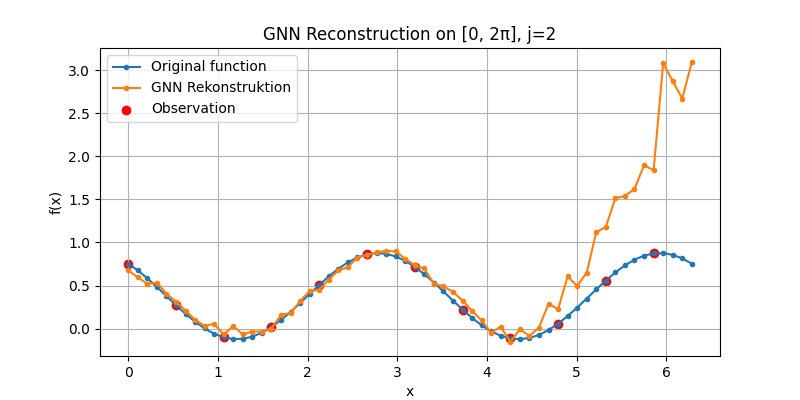
\includegraphics[width=0.23\textwidth]{images/gnn_obs_naive_j2_jj2_0.png} &
    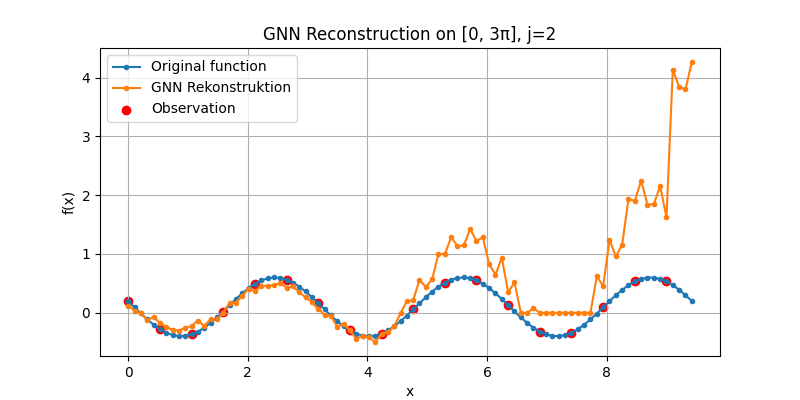
\includegraphics[width=0.23\textwidth]{images/gnn_obs_naive_j2_jj3_0.png} &
    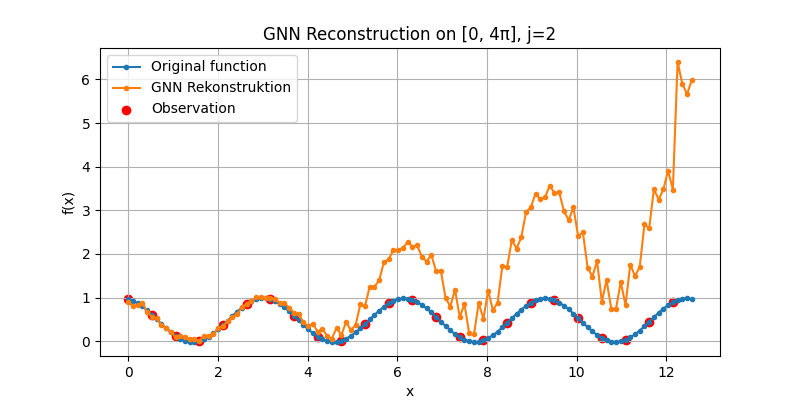
\includegraphics[width=0.23\textwidth]{images/gnn_obs_naive_j2_jj4_0.png} \\
    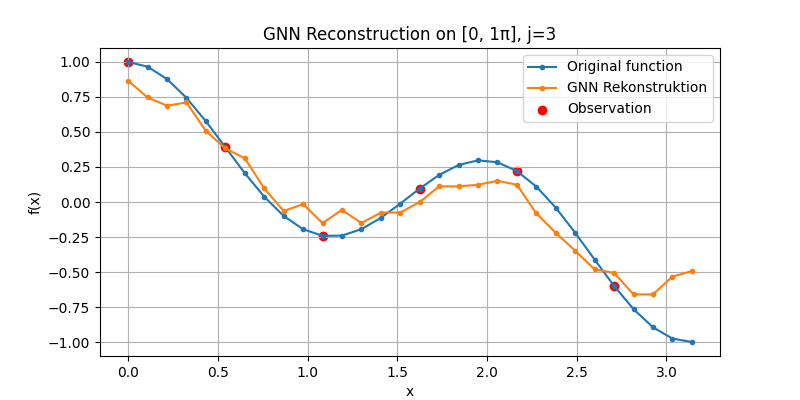
\includegraphics[width=0.23\textwidth]{images/gnn_obs_naive_j3_jj1_0.png} &
    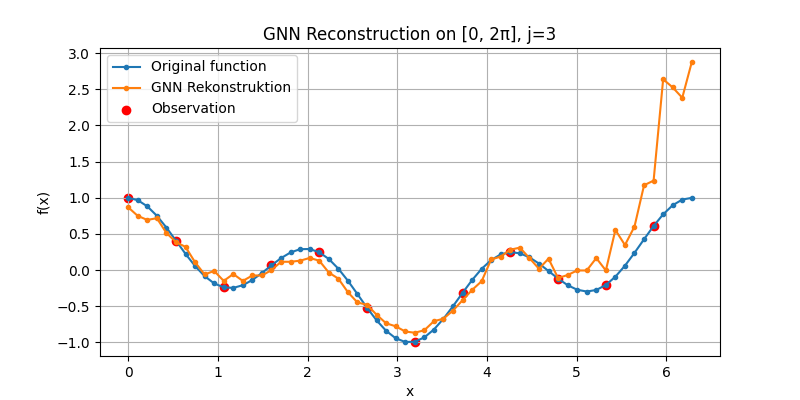
\includegraphics[width=0.23\textwidth]{images/gnn_obs_naive_j3_jj2_0.png} &
    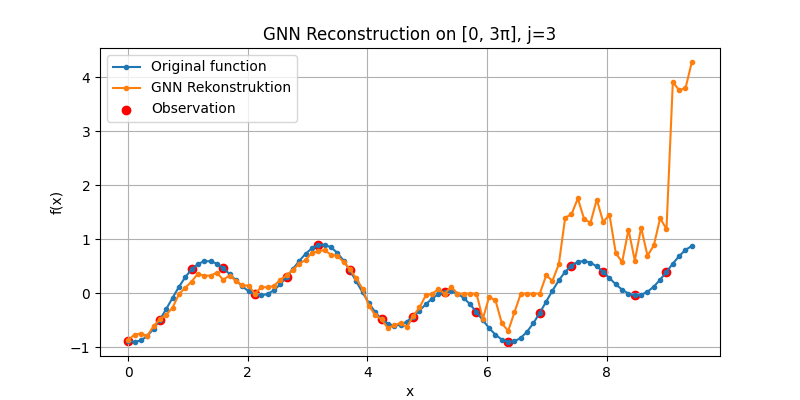
\includegraphics[width=0.23\textwidth]{images/gnn_obs_naive_j3_jj3_0.png} &
    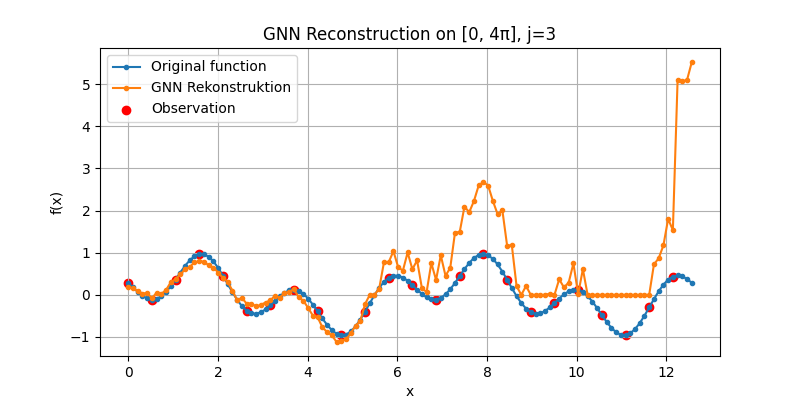
\includegraphics[width=0.23\textwidth]{images/gnn_obs_naive_j3_jj4_0.png} \\
    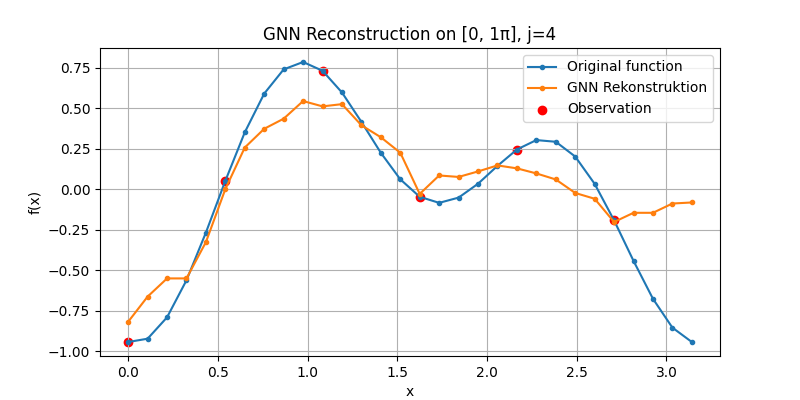
\includegraphics[width=0.23\textwidth]{images/gnn_obs_naive_j4_jj1_0.png} &
    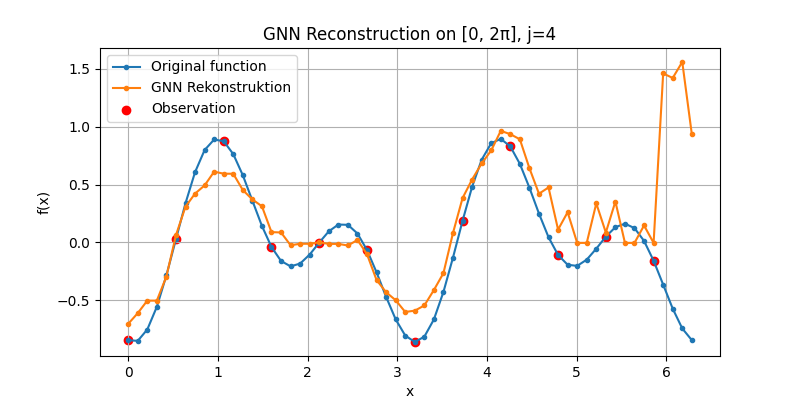
\includegraphics[width=0.23\textwidth]{images/gnn_obs_naive_j4_jj2_0.png} &
    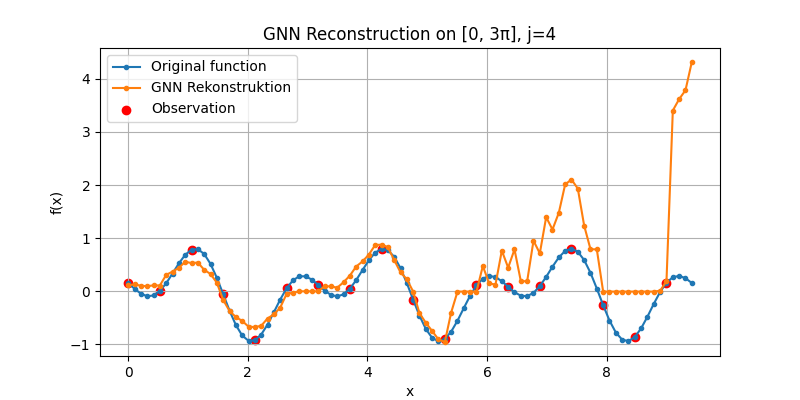
\includegraphics[width=0.23\textwidth]{images/gnn_obs_naive_j4_jj3_0.png} &
    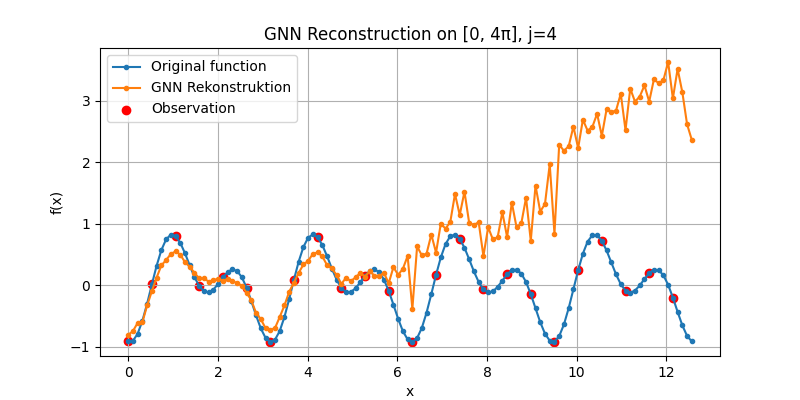
\includegraphics[width=0.23\textwidth]{images/gnn_obs_naive_j4_jj4_0.png} \\
  \end{tabular}
  \caption{GNN reconstruction results for functions $f(x) = \cos(x + \phi)\cos((j-1)x)$ with increasing frequency ($j = 1$ to $4$) and interval length ($jj = 1$ to $4$). Each image shows prediction based on sparse observations.}
  \label{fig:gnn_jj_generalization_full}
\end{figure}


\paragraph{Step 5: Testing on Extended Domains}

We evaluate the trained model on functions of the form $f(x) = \cos(x + \phi)\cos((j-1)x)$ over extended intervals $[0, j \cdot \pi]$. This tests the generalization ability of the GNN.

\begin{codeonly}{Test Function and Evaluation}
def run_test(j, jj):
    N_test = jj * 30
    x_test_grid = torch.linspace(0, jj * np.pi, N_test)

    phi_test = torch.rand(1).item() * np.pi
    f_test = lambda x: torch.cos(x + phi_test) * torch.cos((j - 1) * x)
    y_test = f_test(x_test_grid)

    mask = torch.zeros(N_test)
    mask[::M] = 1.0
    obs = y_test * mask
    x_feat_test = torch.stack([x_test_grid, obs, mask], dim=1)

    edges = []
    for i in range(N_test):
        edges.append((i, i))  # Self-loop
        for k in range(1, K + 1):
            if i - k >= 0:
                edges.append((i, i - k))
            if i + k < N_test:
                edges.append((i, i + k))
    edge_index_test = torch.tensor(edges).T

    model.eval()
    with torch.no_grad():
        pred_test = model(x_feat_test, edge_index_test)

    plt.figure(figsize=(8, 4))
    plt.plot(x_test_grid, y_test, '.-', label="Original function")
    plt.plot(x_test_grid, pred_test, '.-', label="GNN Rekonstruktion")
    plt.scatter(x_test_grid[::M], y_test[::M], color='red', label="Observation")
    plt.title(f"GNN Reconstruction on [0, {jj}pi], j={j}")
    plt.xlabel("x")
    plt.ylabel("f(x)")
    plt.grid(True)
    plt.legend()
    plt.show()

for j in range(1, 5):
    run_test(1, jj=j)
    run_test(j, jj=j)
\end{codeonly}

\paragraph{Conclusion}

This naive setup already demonstrates the capacity of GNNs to reconstruct continuous functions from sparse data. In the next sections, we will explore how to generalize this setup and test whether absolute positional information (i.e., $x$) is truly necessary for accurate reconstructions.

%==============================================================================
%
%==============================================================================
\subsection{Coordinate-Free GNN: Learning from Observations Alone}

In this variation, we explore the idea of removing the coordinate $x$ from the GNN input entirely. Instead of feeding the spatial location explicitly into the model, we rely solely on two pieces of information per node:
\begin{itemize}
  \item the observed function value (or zero if unobserved),
  \item a binary mask indicating whether the value was observed.
\end{itemize}
The graph topology itself continues to encode spatial relationships via $K$-nearest neighbors. This setup allows the network to learn purely from **relational** and **structural** information.

\vspace{0.5em}
\noindent
To implement this, we change the input feature dimension to 2 and remove $x$ from the input vector:

\begin{codeonly}{Model Without Coordinates}
class GNN(nn.Module):
    def __init__(self, in_dim=2, hidden=64):
        ...
x_feat = torch.stack([obs_y, mask], dim=1)  # No x-coordinate
model2 = GNN(in_dim=2)
\end{codeonly}

\vspace{0.5em}
\noindent
The training loop remains identical. For testing, we run the same function `run\_test(j, jj, tag)` but again exclude the coordinate $x$ from the input:

\begin{codeonly}{Coordinate-Free Testing}
x_feat_test = torch.stack([obs, mask], dim=1)
pred_test = model2(x_feat_test, edge_index_test)
plt.savefig(f"gnn_obs_no_pos_j{j}_jj{jj}_{tag}.png")
\end{codeonly}


\begin{figure}[ht]
  \centering
  \begin{tabular}{cccc}
    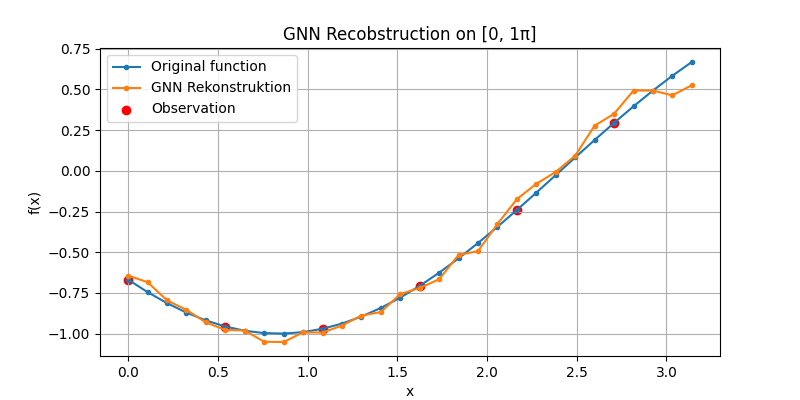
\includegraphics[width=0.23\textwidth]{images/gnn_obs_no_pos_j1_jj1_0.png} &
    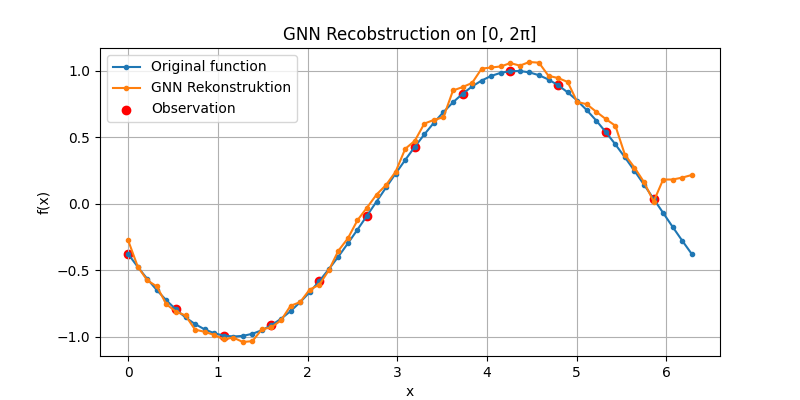
\includegraphics[width=0.23\textwidth]{images/gnn_obs_no_pos_j1_jj2_0.png} &
    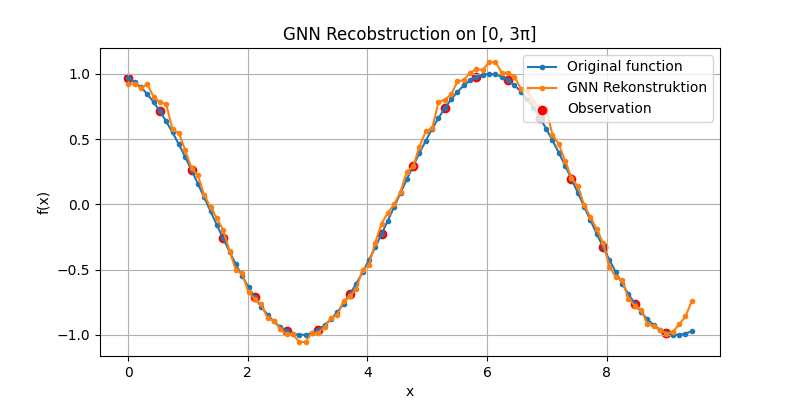
\includegraphics[width=0.23\textwidth]{images/gnn_obs_no_pos_j1_jj3_0.png} &
    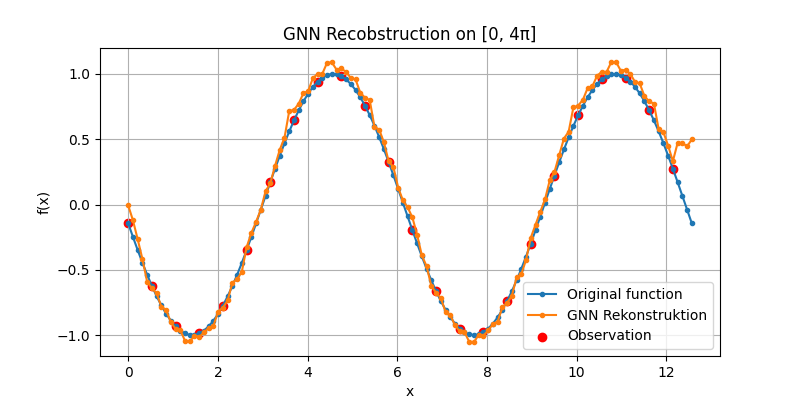
\includegraphics[width=0.23\textwidth]{images/gnn_obs_no_pos_j1_jj4_0.png} \\
    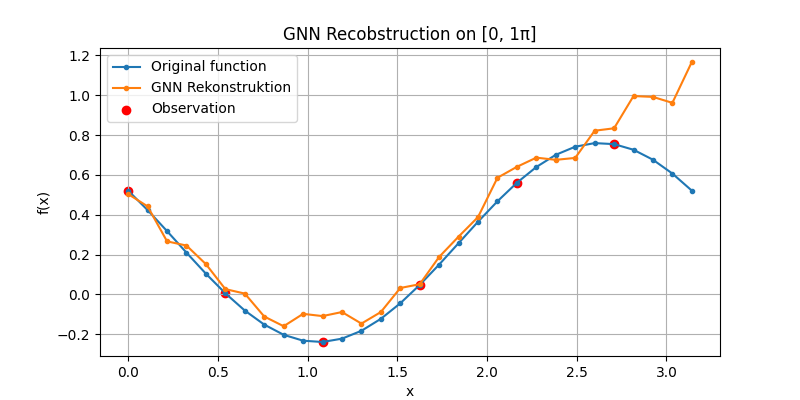
\includegraphics[width=0.23\textwidth]{images/gnn_obs_no_pos_j2_jj1_0.png} &
    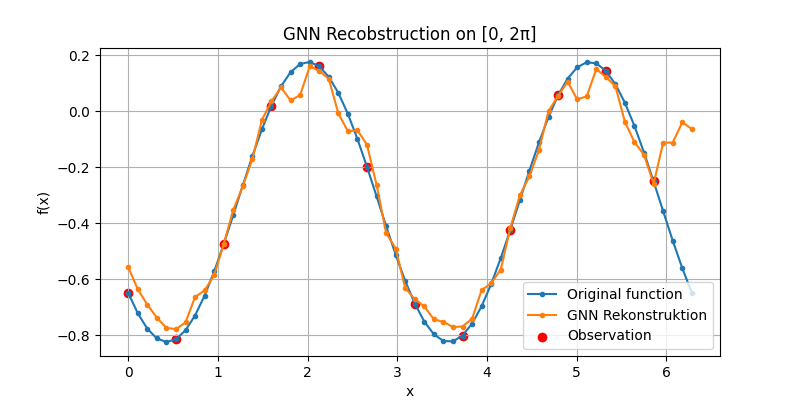
\includegraphics[width=0.23\textwidth]{images/gnn_obs_no_pos_j2_jj2_0.png} &
    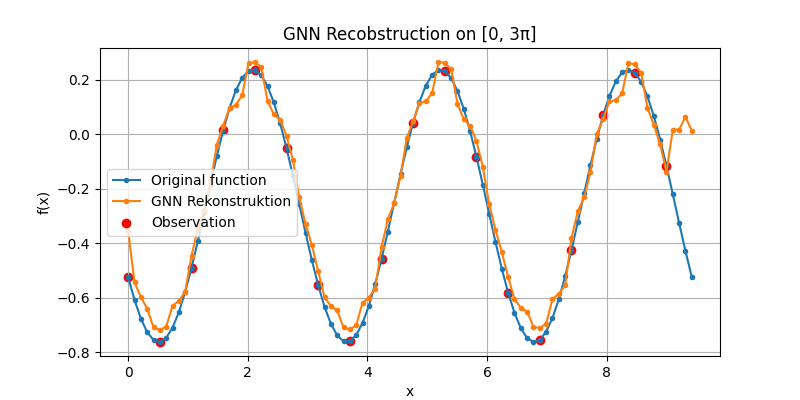
\includegraphics[width=0.23\textwidth]{images/gnn_obs_no_pos_j2_jj3_0.png} &
    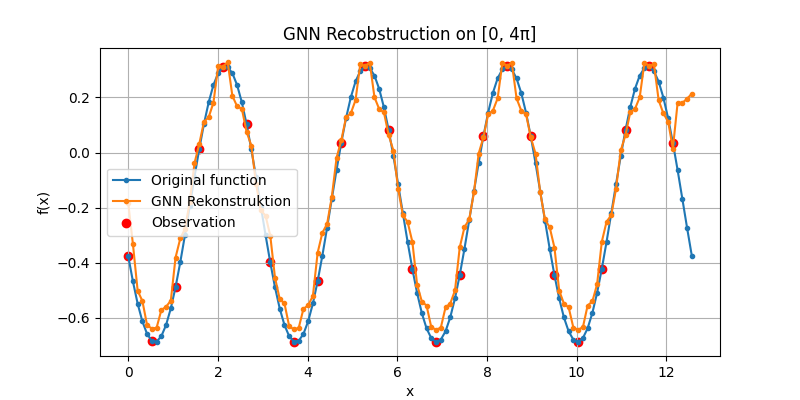
\includegraphics[width=0.23\textwidth]{images/gnn_obs_no_pos_j2_jj4_0.png} \\
    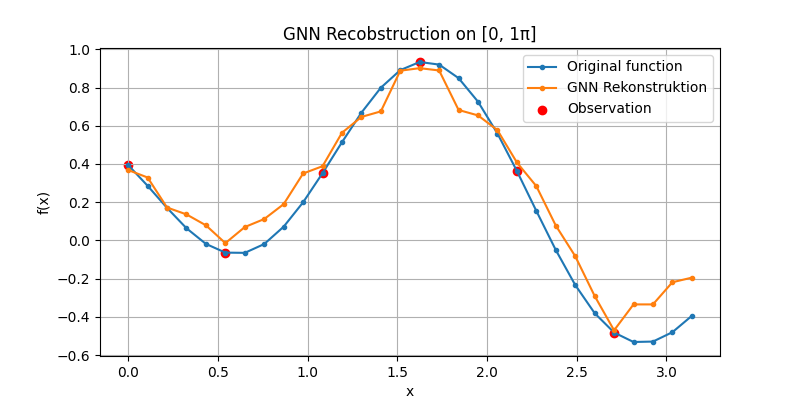
\includegraphics[width=0.23\textwidth]{images/gnn_obs_no_pos_j3_jj1_0.png} &
    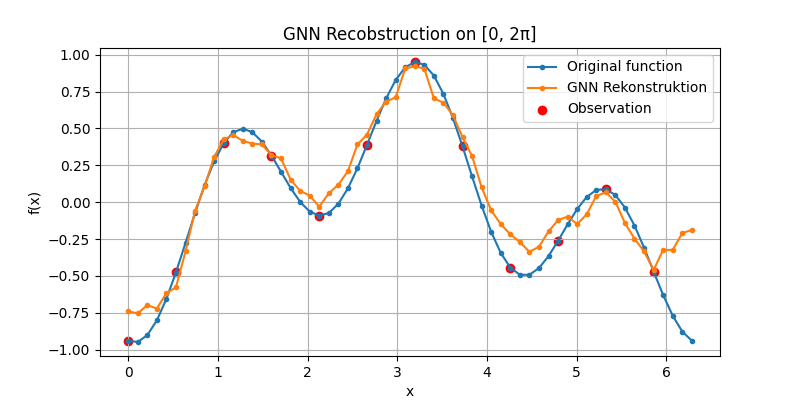
\includegraphics[width=0.23\textwidth]{images/gnn_obs_no_pos_j3_jj2_0.png} &
    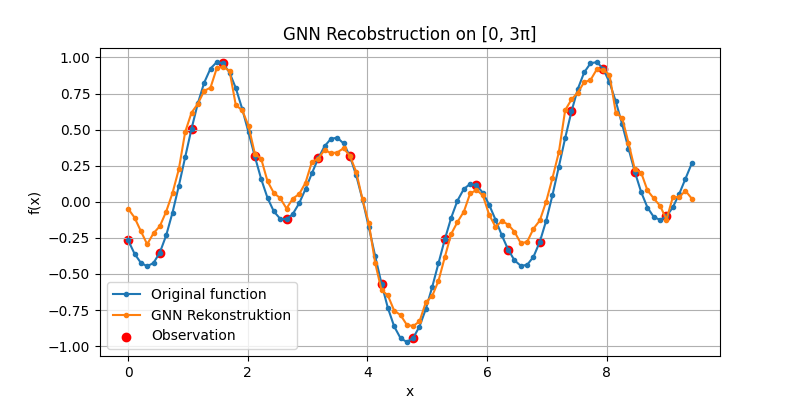
\includegraphics[width=0.23\textwidth]{images/gnn_obs_no_pos_j3_jj3_0.png} &
    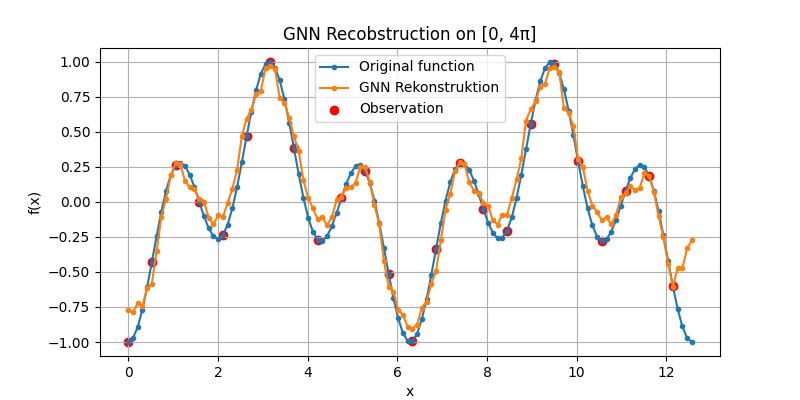
\includegraphics[width=0.23\textwidth]{images/gnn_obs_no_pos_j3_jj4_0.png} \\
    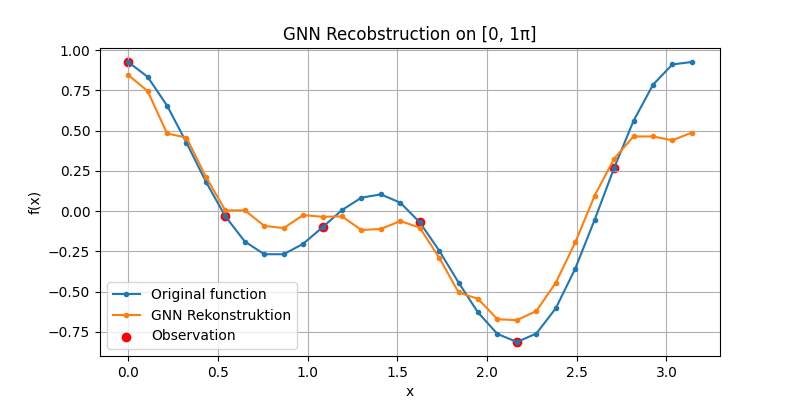
\includegraphics[width=0.23\textwidth]{images/gnn_obs_no_pos_j4_jj1_0.png} &
    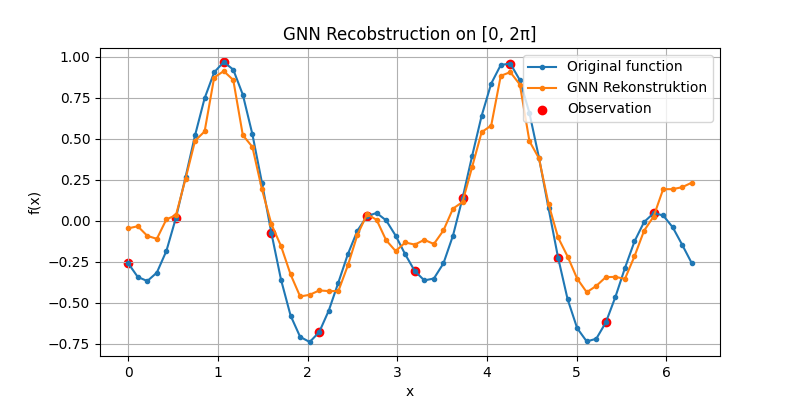
\includegraphics[width=0.23\textwidth]{images/gnn_obs_no_pos_j4_jj2_0.png} &
    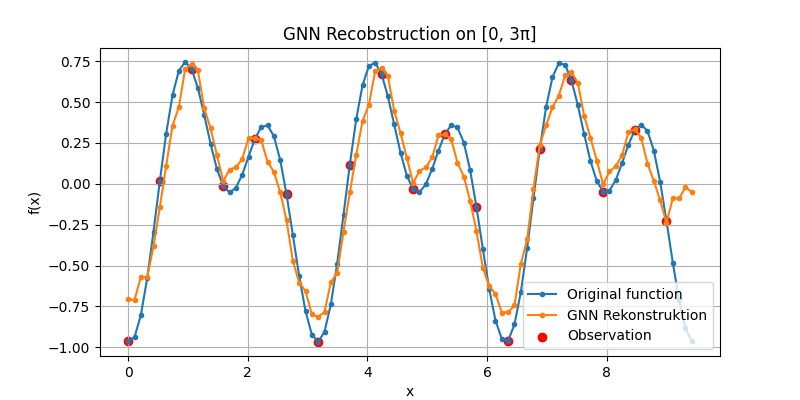
\includegraphics[width=0.23\textwidth]{images/gnn_obs_no_pos_j4_jj3_0.png} &
    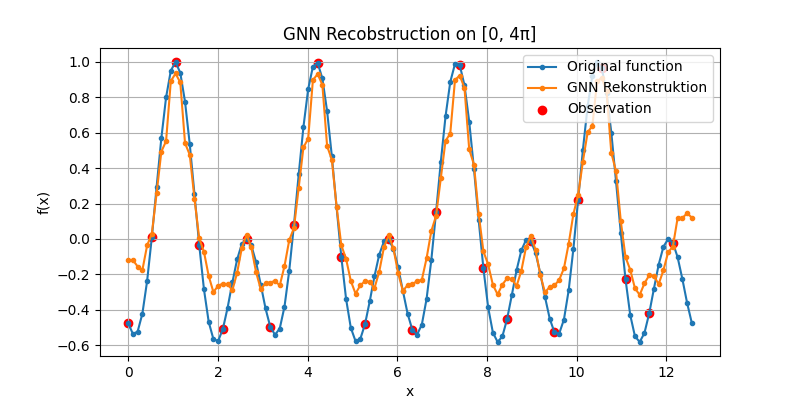
\includegraphics[width=0.23\textwidth]{images/gnn_obs_no_pos_j4_jj4_0.png} \\
  \end{tabular}
  \caption{GNN reconstructions without coordinate input. Each panel shows $f(x) = \cos(x + \phi)\cos((j-1)x)$ reconstructed from sparse observations, across increasing frequency $j = 1\ldots4$ and domain size $jj = 1\ldots4$. The model was trained without using $x$-position as input and on shifted sines only, no higher modes in the training dataset.}
  \label{fig:gnn_no_pos_grid}
\end{figure}

\paragraph{Surprising Result: Better Generalization Without Coordinates}

This variant performs {\em significantly better} when generalizing to longer domains and higher-frequency functions. While this may appear counterintuitive at first, the reason is rooted in how the model interprets the coordinate input.

When $x$ is included as a feature, the GNN must learn to "undo" the fact that $x$ changes range across intervals. For example, $x \in [0,\pi]$ during training but later $x \in [0,4\pi]$ during testing — unless the network has learned that $x$ is irrelevant, it may overfit to this scale and fail to generalize.

By removing $x$, we force the network to focus on {\bf local patterns} and {\bf relational geometry} encoded in the graph structure — which remains scale-invariant and consistent across test domains.

%==============================================================================
%
%==============================================================================
\section{Exploring Graph Structures in Detail}

\subsection{Inspecting the Number of Trainable Parameters}

Graph neural networks (GNNs) operate on graph-structured data by aggregating and transforming node features according to a given graph topology. The structure of the graph is provided through the {\tt edge\_index}, which specifies the connections between nodes, while the trainable parameters of the model are applied uniformly across the entire graph.

\begin{codeonly}{Edge Index and GNN Forward Pass}
# x: [N, F] feature matrix for N nodes, each with F features
# edge_index: [2, E] matrix with E directed edges (source, target)

x = model(x, edge_index)
\end{codeonly}

The {\tt edge\_index} is a $2 \times E$ tensor that defines the spatial structure of the graph by listing all $E$ edges as source-target pairs. It governs how information flows between nodes, but it does not introduce any additional trainable parameters. Instead, the weights in a GNN are shared across all nodes and edges, making the model invariant to the graph size and applicable to different domains.

Each layer in the model—such as linear projections and message-passing operations—has its own set of parameters, which are learned during training. These parameters determine {\bf how} node features are updated, while the {\tt edge\_index} determines {\bf where} messages are exchanged. As a result, we can reuse the same trained model architecture and weights on graphs of varying size or structure, as long as the input feature format remains consistent.

{\bf Parameter Numbers.} We now explore the exact number of trainable parameters in our models using a simple Python function and interpret how input dimensionality affects model complexity.

To measure the size of a model, we compute the total number of trainable parameters using the function {\tt nelement()} for each parameter tensor. The command shown sums over all layers and returns a single integer that quantifies the model's capacity.

\begin{codeonly}{One Linear Model Parameters}
sum([param.nelement() for param in model.parameters()])
\end{codeonly}

To inspect the complexity of our models, we define a simple Python function that iterates over all trainable parameters and prints their names, shapes, and counts:

\begin{codeonly}{Simple Parameter Summary}
def simple_param_summary(model):
    print('-'*80)
    total = 0
    print("Layer Summary:")
    for name, param in model.named_parameters():
        count = param.numel()
        total += count
        print(f"{name:30} | shape: {list(param.shape)} | params: {count}")
    print(f"\nTotal trainable parameters: {total}")
\end{codeonly}

This function produces an informative overview, showing the parameter count for each layer and the overall model. We apply it to two model variants: {\bf model}, which uses the full feature vector \texttt{[x, val, mask]} with input dimension 3, and {\bf model2}, which omits the coordinate and uses only \texttt{[val, mask]} with input dimension 2.

\vspace{1em}
{\bf Result for model (with coordinate):}

\begin{verbatim}
input_proj.weight              | shape: [64, 3] | params: 192
input_proj.bias                | shape: [64]    | params: 64
gnn1.self_lin.weight           | shape: [64, 64] | params: 4096
gnn1.self_lin.bias             | shape: [64]     | params: 64
gnn1.neigh_lin.weight          | shape: [64, 64] | params: 4096
gnn1.neigh_lin.bias            | shape: [64]     | params: 64
gnn2.self_lin.weight           | shape: [64, 64] | params: 4096
gnn2.self_lin.bias             | shape: [64]     | params: 64
gnn2.neigh_lin.weight          | shape: [64, 64] | params: 4096
gnn2.neigh_lin.bias            | shape: [64]     | params: 64
out.weight                     | shape: [1, 64]  | params: 64
out.bias                       | shape: [1]      | params: 1
Total trainable parameters: 16961
\end{verbatim}

\vspace{1em}
{\bf Result for model2 (without coordinate):}

\begin{verbatim}
input_proj.weight              | shape: [64, 2] | params: 128
input_proj.bias                | shape: [64]    | params: 64
... (identical hidden layers and output)
Total trainable parameters: 16897
\end{verbatim}

The only difference lies in the first linear layer. With three input features, the input projection layer has $64 \times 3 + 64 = 256$ parameters, while with two inputs it has $64 \times 2 + 64 = 192$ parameters. This difference of exactly 64 parameters matches the total discrepancy between the models.

\vspace{1em}
{\bf Interpretation:} The rest of the model—two GNN layers with shared hidden size and the final output projection—remains identical in both cases. This small change in input dimensionality helps us isolate the effect of using or omitting positional information ($x$) while keeping model capacity nearly the same.

This method is a convenient way to audit model size, debug unexpected parameter growth, or document the impact of architectural choices.

%==============================================================================
%
%==============================================================================
\subsection{Marching through the Graph Processing}

\begin{figure}[ht]
    \centering
    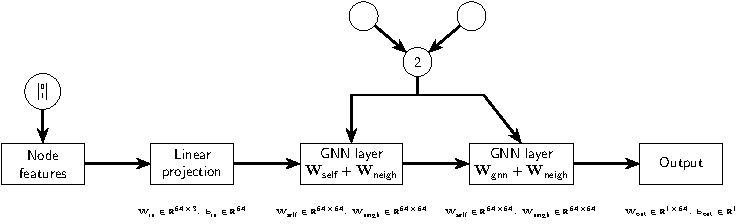
\includegraphics[width=\textwidth]{images/graph_structure.pdf}
    \caption{Schematic of the GNN architecture with input projection, two GNN layers using neighborhood aggregation, and output transformation.}
    \label{fig:gnn-structure}
\end{figure}

%------------------------------------------------------------------------------
%
%------------------------------------------------------------------------------
{\bf Step 1: Raw Node Input Features.} Each node $i$ in the graph carries basic local information encoded as a 2-dimensional vector:
\[
\mathbf{x}_i^{(0)} =
\begin{bmatrix}
\mathrm{val}_i \\
\mathrm{mask}_i
\end{bmatrix} \in \mathbb{R}^2.
\]

This input consists of:
\begin{itemize}
  \item $\mathrm{val}_i$: the observed function value at the node $i$, or $0$ if the value is unobserved,
  \item $\mathrm{mask}_i \in \{0, 1\}$: a binary indicator specifying whether the value is present ($1$) or missing ($0$).
\end{itemize}

The full input feature matrix for all $N$ nodes in the graph is:
\[
X^{(0)} =
\begin{bmatrix}
--- & \mathbf{x}_1^{(0)} & --- \\
--- & \mathbf{x}_2^{(0)} & --- \\
& \vdots & \\
--- & \mathbf{x}_N^{(0)} & ---
\end{bmatrix}
\in \mathbb{R}^{N \times 2}.
\]

\medskip
{\bf Motivation:} This minimal feature representation provides the model with:
\begin{itemize}
  \item The available measurement data (only at selected nodes),
  \item An explicit signal of which nodes are observed and which are not,
  \item A compact and domain-agnostic encoding that avoids absolute positional information.
\end{itemize}

\medskip
These raw inputs are passed to the first learnable layer of the network — the linear projection — which maps them into a higher-dimensional latent space for further processing and message passing.


%------------------------------------------------------------------------------
%
%------------------------------------------------------------------------------
{\bf Step 2: Linear Input Projection Layer.} Each node in the graph is initially represented by a 2-dimensional feature vector:
\[
\mathbf{x}_i^{(0)} = 
\begin{bmatrix}
\mathrm{val}_i \\
\mathrm{mask}_i
\end{bmatrix}
\in \mathbb{R}^2,
\]
where
\begin{itemize}
  \item $\mathrm{val}_i$ is the observed function value at node $i$ (or zero if unobserved),
  \item $\mathrm{mask}_i \in \{0, 1\}$ indicates whether the observation is present.
\end{itemize}

These raw features are passed through a learned linear transformation to project them into a higher-dimensional feature space:
\[
\mathbf{x}_i^{(1)} = \sigma\left( W \mathbf{x}_i^{(0)} + \mathbf{b} \right), \quad W \in \mathbb{R}^{64 \times 2}, \quad \mathbf{b} \in \mathbb{R}^{64},
\]
where $\sigma$ is the ReLU activation function applied component-wise:
\[
\sigma(z) = \max(0, z).
\]

This operation is applied independently to all $N$ nodes in the graph, resulting in a projected feature matrix
\[
X^{(1)} \in \mathbb{R}^{N \times 64}.
\]

\medskip
{\bf Purpose:} This step enables the model to:
\begin{itemize}
  \item Interpret the semantic meaning of the raw inputs,
  \item Learn different representations for observed and unobserved nodes,
  \item Embed all nodes into a common latent space for message passing.
\end{itemize}

\medskip
{\bf Interpretation:} The weights in $W$ determine how much influence the observed value and the mask have on each of the 64 embedding dimensions. For example:
\begin{itemize}
  \item Some dimensions may be dominated by the presence or absence of data,
  \item Others may capture approximate magnitudes or trends across the domain.
\end{itemize}

This projected representation is then passed to the GNN layers, where it is refined through interaction with neighboring nodes.

%------------------------------------------------------------------------------
%
%------------------------------------------------------------------------------
{\bf Step 3: Message Passing with GNNLayer.} After the input features have been projected to the latent space $\mathbb{R}^{64}$, the node embeddings are updated using the graph structure. This happens through two successive {\tt GNNLayer} blocks, each of which applies message passing followed by a learned transformation.

For the first layer, the input is $X^{(1)} \in \mathbb{R}^{N \times 64}$. The message passing operation updates each node $i$ based on its own features and the features of its neighbors, as defined by the edge list {\tt edge\_index}.

\medskip
Each {\tt GNNLayer} performs the following update:
\[
\mathbf{x}_i^{(\ell+1)} = \sigma\left(
W_{\text{self}} \mathbf{x}_i^{(\ell)} +
W_{\text{neigh}} \sum_{j \in \mathcal{N}(i)} \mathbf{x}_j^{(\ell)}
\right),
\]
where:
\begin{itemize}
  \item $\mathbf{x}_i^{(\ell)} \in \mathbb{R}^{64}$ is the node feature vector at layer $\ell$,
  \item $\mathcal{N}(i)$ is the set of neighbors of node $i$ (including self-loop),
  \item $W_{\text{self}}, W_{\text{neigh}} \in \mathbb{R}^{64 \times 64}$ are learned weight matrices,
  \item $\sigma$ is the ReLU activation function.
\end{itemize}

The neighborhood aggregation is computed via:
\[
\mathbf{a}_i = \sum_{j \in \mathcal{N}(i)} \mathbf{x}_j^{(\ell)},
\]
which is then linearly transformed and added to the transformed self-information. In PyTorch, this is implemented by accumulating neighbor features with the operation:
\begin{verbatim}
agg = torch.zeros_like(x)
agg.index_add_(0, row, x[col])
\end{verbatim}
where {\tt edge\_index = [row, col]} encodes all directed edges from node {\tt col[k]} to node {\tt row[k]}.

\medskip
{\bf Interpretation:} This layer learns how to combine a node's own state with information from its local neighborhood. It does so in a trainable, nonlinear way, which enables it to reconstruct smooth or structured functions based on sparsely observed values.

Two such GNN layers are applied in sequence in the model, each refining the representation based on a wider receptive field (i.e., information from nodes up to two hops away).

%------------------------------------------------------------------------------
%
%------------------------------------------------------------------------------
{\bf Step 4: Output Projection.} After two rounds of message passing, each node $i$ is represented by a refined hidden state vector:
\[
\mathbf{x}_i^{(3)} \in \mathbb{R}^{64}.
\]

To convert this latent representation into a scalar prediction (e.g., an estimate of the underlying function value at node $i$), the model applies a final linear projection:
\[
\hat{y}_i = w^\top \mathbf{x}_i^{(3)} + b,
\quad w \in \mathbb{R}^{64}, \quad b \in \mathbb{R}.
\]

This is implemented in PyTorch as:
\begin{verbatim}
self.out = nn.Linear(64, 1)
\end{verbatim}

Applied to all $N$ nodes, the output becomes:
\[
\hat{y} =
\begin{bmatrix}
\hat{y}_1 \\
\hat{y}_2 \\
\vdots \\
\hat{y}_N
\end{bmatrix}
\in \mathbb{R}^{N},
\]
which is compared to the true function $y \in \mathbb{R}^{N}$ during training using a mean squared error loss:
\[
\mathcal{L} = \frac{1}{N} \sum_{i=1}^N (\hat{y}_i - y_i)^2.
\]

\medskip
{\bf Purpose:} This step transforms the latent node embedding back into the physical space of scalar function values. It completes the reconstruction process by producing a prediction for every node in the graph — observed or not.

\medskip
{\bf Interpretation:} The model learns to extract the relevant features through the graph structure and to compress them into a meaningful final scalar output. Since the same output transformation is applied to every node, the model remains fully permutation-invariant with respect to the node order.

\medskip
{\bf Final Remarks on Structure and Complexity.}
The graph network architecture described in this section is compact yet expressive. It processes node-wise inputs in four clearly structured stages as shown in Figure \ref{fig:gnn-structure}: 
\begin{itemize}
\item
input feature encoding, 
\item
projection into a latent space, 
\item
two rounds of message passing, and 
\item
a final output projection. 
\end{itemize}
Each {\tt GNNLayer} updates node representations by combining a self-weighted embedding with a shared transformation of its neighbors — using just two weight matrices per layer, independent of the graph's size or shape. 

The total number of parameters remains modest (16{,}961 in the case of three input features), with the majority concentrated in the two GNN layers. Despite this simplicity, the model captures complex interactions across the graph and generalizes naturally to different domains. Crucially, the graph structure itself is not learned but provided externally via {\tt edge\_index}, making the model both interpretable and highly adaptable. This layered design, along with consistent weight sharing and localized aggregation, gives the network its power to generalize, interpolate, and reconstruct global behavior from sparse, local input.


%==============================================================================
%
%==============================================================================
\section{PyTorch Lightning and PyTorch Geometric}

Modern PyTorch workflows benefit greatly from using helper libraries that simplify model training and extend PyTorch with domain-specific components. Two such libraries are:

\begin{itemize}
  \item {\bf PyTorch Lightning:} A high-level wrapper around PyTorch that structures training, logging, and hardware management into a clean and scalable format.
  \item {\bf PyTorch Geometric (PyG):} A specialized library for graph neural networks (GNNs), enabling message passing, pooling, and graph data structures.
\end{itemize}

These libraries integrate seamlessly and can be used together to train graph-based models in a clean and efficient way.

To follow the examples in this tutorial, the following packages must be installed. Installation should be done in a Python 3.9+ environment with PyTorch already installed.

\begin{codeonly}{Installation via pip}
pip install pytorch-lightning
pip install torch-geometric
pip install torch-scatter torch-sparse torch-cluster
\end{codeonly}

{\bf PyTorch Lightning} and {\bf PyTorch Geometric} are two independent libraries, both built on top of PyTorch:
\begin{itemize}
  \item PyTorch Lightning simplifies model training, logging, and hardware management, but is agnostic to the model type.
  \item PyTorch Geometric specializes in graph data structures and operations, enabling message-passing networks and geometric deep learning.
\end{itemize}

You can use either library independently or combine them:
\begin{itemize}
  \item PyG can be used alone to build and train GNNs using a manual training loop.
  \item Lightning can be used to train any model, including non-graph models like CNNs, RNNs, or transformers.
  \item Using both together is ideal for clean training of graph models at scale, with integrated logging and device handling.
\end{itemize}

\vspace{1em}

\begin{center}
\begin{tabular}{|l|c|c|c|}
\hline
{\bf Use Case} & {\bf PyG only} & {\bf Lightning only} & {\bf PyG + Lightning} \\
\hline
Small GNN script              & \checkmark & --         & optional \\
General ML model training     & --         & \checkmark & optional \\
Large graph model w/ logging  & \checkmark & \checkmark & \checkmark (recommended) \\
Clean training loop           & --         & \checkmark & \checkmark \\
Graph-specific layers         & \checkmark & --         & \checkmark \\
\hline
\end{tabular}
\end{center}

This tutorial demonstrates both libraries separately and together, helping you choose the best level of abstraction for your needs.

%------------------------------------------------------------------------------
%
%------------------------------------------------------------------------------
\subsection{A PyTorch Lightning Example}

As a first example of PyTorch Lightning, we define a regression task where the model learns to reconstruct a shifted sine function from a sparse set of observations. Each sample is a 1D graph of points connected to their 3 nearest neighbors to the left and right. Node features include both the (possibly missing) observed values and a binary observation mask.

%------------------------------------------------------------------------------
%
%------------------------------------------------------------------------------
\begin{figure}[ht]
    \centering
    \includegraphics[width=0.6\textwidth]{images/lightning_demo.png}
    \caption{%
        Graph neural network interpolation of a shifted sine function using PyTorch Lightning and PyTorch Geometric.
        The model observes only a small subset of values (red dots) and learns to reconstruct the full curve (orange dashed line).
        The ground truth is shown as a solid blue line.
    }
    \label{fig:gnn-sine-interpolation}
\end{figure}

%------------------------------------------------------------------------------
%
%------------------------------------------------------------------------------
{\bf Data Generation.} We generate sine curves with random phase shifts and mask most values. Each graph stores the full target \texttt{y}, the sparse observation vector \texttt{y\_obs}, and a 2-channel input feature vector.

\begin{codeonly}{Sine Graph with Observation Mask}
def generate_sample_graph(n_nodes=64, dn=8, k=3):
    x_vals = torch.linspace(0, 2 * np.pi, n_nodes)
    phase = np.random.uniform(0, 2 * np.pi)
    y_true = torch.sin(x_vals + phase)

    y_obs = torch.full_like(y_true, float('nan'))
    idx = torch.arange(0, n_nodes, dn)
    y_obs[idx] = y_true[idx]

    is_observed = ~torch.isnan(y_obs)
    input_feat = torch.stack([
        torch.nan_to_num(y_obs, nan=0.0),
        is_observed.float()
    ], dim=1)

    edges = []
    for i in range(n_nodes):
        for j in range(1, k + 1):
            if i - j >= 0:
                edges.append((i, i - j))
            if i + j < n_nodes:
                edges.append((i, i + j))
    edge_index = torch.tensor(edges, dtype=torch.long).t().contiguous()

    return Data(x_feat=input_feat, y=y_true.unsqueeze(1), y_obs=y_obs.unsqueeze(1), edge_index=edge_index)
\end{codeonly}

%------------------------------------------------------------------------------
%
%------------------------------------------------------------------------------
{\bf Lightning Model.} The Lightning module uses three GCN layers. The input has two channels (value and mask), and the model is trained to match the true signal where no observations were provided.

\begin{codeonly}{PyTorch Lightning GCN}
class GNNInterpolator(pl.LightningModule):
    def __init__(self):
        super().__init__()
        self.gcn1 = GCNConv(2, 64)
        self.gcn2 = GCNConv(64, 128)
        self.out  = GCNConv(128, 1)

    def forward(self, data):
        x = data.x_feat
        x = F.relu(self.gcn1(x, data.edge_index))
        x = F.relu(self.gcn2(x, data.edge_index))
        return self.out(x, data.edge_index)

    def training_step(self, batch, batch_idx):
        pred = self(batch)
        mask = ~torch.isnan(batch.y_obs)
        loss = F.mse_loss(pred[~mask], batch.y[~mask])
        self.log("train_loss", loss)
        return loss

    def configure_optimizers(self):
        return torch.optim.Adam(self.parameters(), lr=0.01)
\end{codeonly}

%------------------------------------------------------------------------------
%
%------------------------------------------------------------------------------
{\bf Training.} Training is performed using a standard Lightning Trainer:

\begin{codeonly}{Training with Lightning}
model = GNNInterpolator()
trainer = pl.Trainer(max_epochs=200, logger=False, enable_checkpointing=False)
trainer.fit(model, loader)
\end{codeonly}

The trained model generalizes well to new shifted sine curves and accurately reconstructs them from sparse values.


%------------------------------------------------------------------------------
%
%------------------------------------------------------------------------------
\subsection{A PyTorch Geometric Example}

Graph neural networks (GNNs) are well-suited for structured data with local neighborhood dependencies. This example shows how PyTorch Geometric can be used to infer a function—such as a shifted sine curve—from sparse observations using graph convolution layers.

{\bf Graph Structure and Input Features.} Each sample is a graph of 64 nodes uniformly spaced on the interval \([0, 2\pi]\), connected to their 3 left and 3 right neighbors. Each node has two features: the (possibly missing) observation value and a binary mask indicating whether it was observed.

\begin{codeonly}{Data Generation with Graph and Mask}
def generate_sample_graph(n_nodes=64, dn=8, k=3):
    x_vals = torch.linspace(0, 2 * np.pi, n_nodes)
    phase = np.random.uniform(0, 2*np.pi)
    y_true = torch.sin(x_vals + phase)

    y_obs = torch.full_like(y_true, float('nan'))
    idx = torch.arange(0, n_nodes, dn)
    y_obs[idx] = y_true[idx]

    is_observed = ~torch.isnan(y_obs)
    input_feat = torch.stack([
        torch.nan_to_num(y_obs, nan=0.0),
        is_observed.float()
    ], dim=1)

    edges = []
    for i in range(n_nodes):
        for j in range(1, k + 1):
            if i - j >= 0:
                edges.append((i, i - j))
            if i + j < n_nodes:
                edges.append((i, i + j))
    edge_index = torch.tensor(edges, dtype=torch.long).t().contiguous()

    return Data(x_feat=input_feat, y=y_true.unsqueeze(1), y_obs=y_obs.unsqueeze(1), edge_index=edge_index)
\end{codeonly}

%------------------------------------------------------------------------------
%
%------------------------------------------------------------------------------
{\bf GCN Model.} The model consists of three GCN layers applied to the 2-channel input.

\begin{codeonly}{PyTorch Geometric GCN}
class GCNInterpolator(torch.nn.Module):
    def __init__(self):
        super().__init__()
        self.gcn1 = GCNConv(2, 64)
        self.gcn2 = GCNConv(64, 128)
        self.out  = GCNConv(128, 1)

    def forward(self, data):
        x = data.x_feat
        x = F.relu(self.gcn1(x, data.edge_index))
        x = F.relu(self.gcn2(x, data.edge_index))
        return self.out(x, data.edge_index)
\end{codeonly}

%------------------------------------------------------------------------------
%
%------------------------------------------------------------------------------
\begin{figure}[ht]
    \centering
    \includegraphics[width=0.6\textwidth]{images/geometric_demo.png}
    \caption{%
        Function interpolation using a Graph Convolutional Network (GCN) in PyTorch Geometric.
        The model reconstructs a shifted sine curve (blue) from sparse observations (red dots).
        The predicted output (orange dashed line) closely follows the true function, demonstrating the model's ability to infer smooth structures from limited data by leveraging graph connectivity.
    }
    \label{fig:pyg-sine-interpolation}
\end{figure}

%------------------------------------------------------------------------------
%
%------------------------------------------------------------------------------
{\bf Training Loop.} A standard PyTorch training loop is used with MSE loss evaluated only on non-observed points.

\begin{codeonly}{Training Loop}
for epoch in range(100):
    for batch in loader:
        pred = model(batch)
        mask = ~torch.isnan(batch.y_obs)
        loss = F.mse_loss(pred[~mask], batch.y[~mask])
        loss.backward()
        optimizer.step()
        optimizer.zero_grad()
\end{codeonly}

%------------------------------------------------------------------------------
%
%------------------------------------------------------------------------------
{\bf Inference and Visualization.} The trained model can interpolate new sine curves from sparse measurements. A typical output looks like this:

\begin{codeonly}{Plotting Output}
plt.plot(x, true, label="True")
plt.plot(x, pred, label="Predicted", linestyle="--")
plt.scatter(x[obs_mask], obs[obs_mask], color='red', label="Observed")
plt.legend()
\end{codeonly}

